% !TeX spellcheck = hu_HU
% !TeX encoding = UTF-8
% !TeX program = xelatex
\documentclass[11pt,a4paper,oneside]{report}             % Single-side
%\documentclass[11pt,a4paper,twoside,openright]{report}  % Duplex

% thanks to http://tex.stackexchange.com/a/47579/71109

% APA-hoz:
\usepackage{csquotes}

\usepackage{ifxetex}
\usepackage{ifluatex}
\newif\ifxetexorluatex % a new conditional starts as false
\ifnum 0\ifxetex 1\fi\ifluatex 1\fi>0
   \xetexorluatextrue
\fi

\ifxetexorluatex
  \usepackage{fontspec}
\else
  \usepackage[T1]{fontenc}
  \usepackage[utf8]{inputenc}
  \usepackage[lighttt]{lmodern}
  \ttfamily\DeclareFontShape{T1}{lmtt}{m}{it}{<->sub*lmtt/m/sl}{}
\fi

\usepackage[english,magyar]{babel} % Alapértelmezés szerint utoljára definiált nyelv lesz aktív, de később külön beállítjuk az aktív nyelvet.

\usepackage{emptypage} % omit page number on empty pages

%\usepackage{cmap}
\usepackage{amsfonts,amsmath,amssymb} % Mathematical symbols.
%\usepackage[ruled,boxed,resetcount,linesnumbered]{algorithm2e} % For pseudocodes. % beware: this is not compatible with LuaLaTeX, see http://tex.stackexchange.com/questions/34814/lualatex-and-algorithm2e
\usepackage{booktabs} % For publication quality tables for LaTeX
\usepackage{graphicx}

\usepackage{subcaption}

%\usepackage{fancyhdr}
%\usepackage{lastpage}

\usepackage{anysize}
%\usepackage{sectsty}
\usepackage{setspace} % For setting line spacing

\usepackage[unicode]{hyperref} % For hyperlinks in the generated document.
\usepackage{xcolor}
\usepackage{listings} % For source code snippets.

\usepackage[amsmath,thmmarks]{ntheorem} % Theorem-like environments.

\usepackage{stmaryrd}

\usepackage[linesnumbered,ruled,vlined]{algorithm2e}
\usepackage{lscape}
\usepackage{listing}
\usepackage{multirow}
\usepackage{makecell}
\usepackage{xcolor}
\usepackage{colortbl}
\usepackage{arydshln}

\usepackage{pdfpages}

%\usepackage[hang]{caption}

%\singlespacing
\onehalfspacing

\newcommand{\selecthungarian}{
	\selectlanguage{magyar}
	\setlength{\parindent}{2em}
	\setlength{\parskip}{0em}
	\frenchspacing
}

\newcommand{\selectenglish}{
	\selectlanguage{english}
	\setlength{\parindent}{0em}
	\setlength{\parskip}{0.5em}
	\nonfrenchspacing
	\renewcommand{\figureautorefname}{Figure}
	\renewcommand{\tableautorefname}{Table}
	\renewcommand{\partautorefname}{Part}
	\renewcommand{\chapterautorefname}{Chapter}
	\renewcommand{\sectionautorefname}{Section}
	\renewcommand{\subsectionautorefname}{Section}
	\renewcommand{\subsubsectionautorefname}{Section}
}

%\usepackage[numbers]{natbib}
%\usepackage{xspace}
%\usepackage[backend=biber,style=apa,language=magyar]{biblatex}
%\addbibresource{src/bib/mybib.bib}

%\usepackage[natbibapa]{apacite}
%\bibliographystyle{apacite}
%\usepackage{xspace}
%\usepackage{natbib}

%-----------------------------------
% APA hivatkozási rendszer beállítása
\usepackage[
    backend=biber,
    style=apa,
    sortcites=true,
    sorting=nyt,
]{biblatex}

\DeclareFieldFormat{edition}{%
	\ifinteger{#1}
	{#1.\addspace kiad.}
	{#1\addspace kiad.}}


%\DeclareLanguageMapping{hungarian}{hungarian-apa}
\addbibresource{bib/mybib.bib}

\usepackage{tablefootnote}

\usepackage{tikz}
\usepackage{pgfplots}
\pgfplotsset{compat=1.17}



\newcommand{\vikcim}{A generatív mesterséges intelligencia szerepe és használatának kihívásai a nagyvállalati szoftverfejlesztésben} % Cím
\newcommand{\vikdoktipus}{\bsc} % Dokumentum típusa (\bsc vagy \msc)

\newcommand{\vikszerzoVezeteknev}{Szkupien}
\newcommand{\vikszerzoKeresztnev}{Péter}

\newcommand{\vikkonzulensAMegszolitas}{dr.~}
\newcommand{\vikkonzulensAVezeteknev}{Drótos}
\newcommand{\vikkonzulensAKeresztnev}{György}

\newcommand{\vikkonzulensBMegszolitas}{}
\newcommand{\vikkonzulensBVezeteknev}{}
\newcommand{\vikkonzulensBKeresztnev}{}

\newcommand{\vikkonzulensCMegszolitas}{}
\newcommand{\vikkonzulensCVezeteknev}{}
\newcommand{\vikkonzulensCKeresztnev}{}

\newcommand{\szerzoMeta}{\vikszerzoVezeteknev{} \vikszerzoKeresztnev} % egy szerző esetén

% Beállítások magyar nyelvű dolgozathoz
\input{include/thesis-hu}


\input{include/preamble}

% Table of contents and the main text
\begin{document}

\pagenumbering{gobble}

\selectthesislanguage

%Titlepage
\hypersetup{pageanchor=false}
%	The title page
\begin{titlepage}
\begin{center}

Budapesti Corvinus Egyetem

\vspace*{5.3cm}

{\huge \bfseries \vikcim}\\[1.2cm]%[0.8cm]


Informatikai menedzsment szak

\vspace*{5.3cm}

{
	\renewcommand{\arraystretch}{0.85}
	\begin{tabular}{cc}
	 \makebox[7cm]{\emph{\keszitette}} & \makebox[7cm]{\emph{\konzulens}} \\ \noalign{\smallskip}
	 \makebox[7cm]{\szerzo} & \makebox[7cm]{\vikkonzulensA} \\
	  & \makebox[7cm]{\vikkonzulensB} \\
	  & \makebox[7cm]{\vikkonzulensC} \\
	\end{tabular}
}

\vfill
{\large \the\year}
\end{center}
\end{titlepage}
\hypersetup{pageanchor=false}

\selectthesislanguage


%\selectlanguage{magyar}
\pagenumbering{gobble}
%\setlength{\parindent}{0pt}

%--------------------------------------------------------------------------------------
% Nyilatkozat
%--------------------------------------------------------------------------------------
\begin{center}
	\large
	\textbf{NYILATKOZAT\\GENERATÍV MESTERSÉGES INTELLIGENCIA HASZNÁLATÁRÓL}\\
\end{center}

\emph{Szkupien Péter} hallgató kijelentem, hogy az \emph{Informatikai menedzsment} szakon 2025/2026/1 félévben beadott szakdolgozatom elkészítéséhez generatív mesterségesintelligencia-rendszert vagy -szolgáltatást használtam az alábbiak szerint:

\begin{itemize}
	\item A rendszer neve: \emph{OpenAI ChatGPT}, célja: források keresése, összefoglalása
	\item A rendszer neve: \emph{Anthropic Claude}, célja: források BibTeX  bejegyzésének generálása
	\item A rendszer neve: \emph{Google NotebookLM}, célja: interjúk hanganyagának összefoglalása
	\item A rendszer neve: \emph{Google Gemini}, célja: szakdolgozat szövegének utólagos szerkesztése
\end{itemize}

Kijelentem, hogy minden generált tartalmat kritikus szemmel ellenőriztem, és meggyőződtem azok megfelelőségéről, ténybeli pontosságáról és jogszerűségéről.

\thispagestyle{empty}

\vfill
\cleardoublepage

%\selectthesislanguage


\pagenumbering{roman}

% Table of Contents
\tableofcontents%\cleardoublepage

% List of Figures, Tables
\listoffigures\addcontentsline{toc}{chapter}{\listfigurename}\cleardoublepage

\listoftables\addcontentsline{toc}{chapter}{\listtablename}\cleardoublepage

% The main part of the thesis
\pagenumbering{arabic}

% Own content
\chapter{\bevezetes} \label{ch:bevezetes}

Az emberiség fejlődésének történetében megannyi vívmány tekinthető mérföldkőnek. Ha a kellően távoli múltba tekintünk, nagyon különböző mérföldköveket találunk, mint pl. a tűz használata, a kerék feltalálása, a könyvnyomtatás, vagy éppen a gőzgép feltalálása. Noha egyik jelentőségéhez sem férhet kétség, mégis szinte lehetetlen összehasonlítani őket, annyira különböző területeken hoztak áttörést.

Az elmúlt évtizedekben azonban a technológiai fejlődés drámaian felgyorsult: a mérföldkövek már nem évszázadonként, hanem évtizedenként, vagy akár csupán néhány évenként követik egymást, témájukban pedig egyre inkább az informatika köré összpontosulnak. A számítógépek megjelenésétől datált időszak – amit nevezhetünk a digitalizáció korának vagy a negyedik ipari forradalomnak is – számos innovációjáról már most biztosan kijelenthető, hogy valóban megváltoztatta az életünket, ilyen pl. a személyi számítógép (PC), az internet, és az okostelefonok elterjedése. Rengeteg olyan is van azonban, amelyek ugyan hasonló változásokat ígértek, a mából még nem lehet eldönteni, valóban be is váltják-e majd ezeket a várakozásokat, mint pl. a virtuális valóság vagy éppen a blokklánc.

Napjainkban a\textit{ mesterséges intelligencia} (MI) az az újdonság, ami lázban tartja a világot (ez nem puszta személyes megfigyelés, a vonatkozó cégek részvényárfolyamainak szárnyalása elég erős indikátor). Ezen belül is a \textit{generatív mesterséges intelligencia} (GMI) a leglátványosabb, hiszen új tartalmakat képes létrehozni. Legyen szó akár szövegről, akár képről, akár videóról, ezek a gombnyomásra, akár ingyenesen létrejövő tartalmak jellegüket tekintve ugyanolyanok, mint azok, amiket eddig kizárólag emberek állítottak elő.
Míg a korábbi innovációk döntően csupán az emberi erőt cserélték gépi erőre, vagy a monoton, repetitív feladatokat automatizálták, a generatív mesterséges intelligenciával \textit{látszólag} intellektuális, kreatív vagy akár művészi folyamatokban is lecserélhetővé válik az ember. Adódik tehát a kérdés, hogy hogyan hat ennek a technológiának a megjelenése olyan emberi tevékenységekre, amelyek esetében korábban fel sem merülhetett, hogy automatizáljuk.

Ebbe a sorba tartozik a szoftverfejlesztés is, ami éppen az az intellektuális tevékenység, ami segítségével eddig a többi repetitív folyamatot automatizáltuk. Hiába szoftverfejlesztés eredményei maguk a generatív mesterséges intelligencia szoftverek is, azok nemcsak célként, hanem eszközként is szolgálhatnak a szoftverfejlesztésben, felvetve a kérdést, hogy hogyan is változtatja meg a generatív mesterséges intelligencia magát a szoftverfejlesztési folyamatot.

Ezt illetően szélsőséges véleményekkel találkozhatunk. Míg egyesek szerint a mesterséges intelligencia megjelenése (és különösen az általa generált kódok) miatt csak még nagyobb szükség lesz szoftverfejlesztőkre, mások szerint a nem is olyan távoli jövőben a mesterséges intelligencia már a szoftverfejlesztők munkáját is el fogja venni, hiszen olcsóbban fog jobb kódokat generálni.

Mivel mérnökinformatikusként magam is szoftverfejlesztőként dolgozom, különösen foglalkoztat a kérdés. Az elmúlt években az az érzés alakult ki bennem, hogy nem lehet nem találkozni ezzel a technológiával, mindenki erről beszél, és öngerjesztő módon mindenki attól fél, hogy kimarad belőle. Az új, látványos eszközök mögött ugyanakkor gyakran nem látszik kristálytisztán a valódi hozzáadott érték, így könnyen megkérdőjelezhető, megalapozottak-e a témát övező hatalmas várakozások. Ennek a kérdésnek a megválaszolása (már ha egyáltalán lehetséges) természetesen jóval túlmutat egy szakdolgozat keretein, mégis egyértelmű volt számomra, hogy ezt a témát szeretném körüljárni.

Szakdolgozatomban azt vizsgálom, hogyan hat a generatív mesterséges intelligencia a szoftverfejlesztésre. A \textit{Software Development Lifecycle} (SDLC) fázisain keresztül elemzem, az egyes fázisokban mi lehet a szerepe ennek az új technológiának, valamint, hogy ehhez képest hol tart a gyakorlatban az alkalmazása. Külön figyelmet fordítok azokra a körülményekre, amelyek relevánsak lehetnek a technológia alkalmazhatóságát illetően, ideértve a potenciális nehézségeket, amelyek meggátolhatják az elméleti felhasználási lehetőségek gyakorlati megvalósulását.

Munkám több ponton is kapcsolódik az Informatikai menedzsment posztgraduális képzés tanmenetéhez. A \textit{Szervezeti információrendszerek} kurzuson külön előadás foglalkozott a mesterséges intelligencia hatásaival (\textit{„Mesterséges intelligencia: Revolution vagy Hype?”}), míg a szoftverfejlesztés a \textit{Software engineering} tárgynak volt témája. A mesterséges intelligencia jogi és biztonsági aspektusait az \textit{Infokommunikációs jog} és az \textit{Informatikai biztonság} kurzusok tárgyalták.

A dolgozat \ref{ch:hatterismeretek}. fejezetében áttekintem a téma releváns elméleti ismereteit, a szoftverfejlesztést és a generatív mesterséges intelligenciát, valamint a kettő találkozását, illetve röviden áttekintem a szoftverfejlesztés iparágát. A \ref{ch:kutatasmodszertan}. fejezetben vázolom kutatásom módszertanát, ideértve a kutatási kérdéseket és az adatgyűjtés módját. A \ref{ch:eredmenyek}. fejezetben kutatási kérdésenként részletesen ismertetem az eredményeket. Az \ref{ch:kovetkeztetesek}. fejezetben következtetéseket vonok le a kutatási eredményekből, valamint megfogalmazok egy akciótervet a technológia bevezetésére. Végül a \ref{ch:osszegzes}. fejezetben összegzem a dolgozatot.

\chapter{Elméleti áttekintés} \label{ch:hatterismeretek}

Hosszú út vezetett az első szoftverek megjelenésétől a generatív mesterséges intelligencia térhódításáig. Az elmúlt évtizedekben a szoftverfejlesztés területén drámai változások zajlottak le, amelyek alapjaiban formálták át a szakmát és a fejlesztési folyamatokat. A technológiai fejlődés következtében egyre összetettebb rendszerek épültek ki, amelyek kezelése és fejlesztése új megközelítéseket és eszközöket igényelt.

Ebben a fejezetben összefoglalom a szakdolgozat témájához kapcsolódó elméleti ismereteket. A \ref{sec:szoftverfejlesztes}. alfejezetben áttekintem a szoftverfejlesztési folyamat lépéseit és fontosabb módszertanait. A \ref{sec:mi}. alfejezetben bemutatom a mesterséges intelligencia főbb területeit. Végül a \ref{sec:mi-fejl}. alfejezetben ismertetem, hogyan hat a mesterséges intelligencia a szoftverfejlesztésre.

\section{Szoftverfejlesztés}\label{sec:szoftverfejlesztes}

A számítógépek fejlődésével egyre bonyolultabb problémák kerültek a programozók látókörébe, hiszen a növekvő számítási kapacitás egyre több esetben volt már elegendő. Ez a potenciál nem is maradt kihasználatlanul, ami a szoftverrendszerek komplexitásának drámai növekedéséhez vezetett \parencite{Briggs02042020}. A kezdeti komplexitást jól mutatja, hogy az első elektronikusan tárolt program, amit Tom Kilburn írt 1948-ban egy szám legnagyobb valódi osztójának megkeresésére, mindössze 17 utasításból állt \parencite{lavington1998history}. Ezzel szemben a Google összes szoftverének együttes kódbázisát 2 milliárd sorosra becsülik \parencite{googlecodebase}, ami jól mutatja a robbanásszerű fejlődést.

A kevesebb, mint egy évszázad alatt ilyen meredeken növekvő bonyolultságot látva nem szabad azonban szem elől tévesztenünk, hogy az emberi agy kapacitása nem változott. Vagyis a szoftveresen megoldott problémák komplexitása bőven átlépte már azt a határt, amit egy ember még részleteiben képes átlátni. Ennek a kezelését az újabb és újabb absztrakciós szintek bevezetése tette lehetővé, hiszen a magasabb absztrakciós szinteken már nem nehezítik a tisztánlátást az alacsonyabb szintek részletei. A növekvő komplexitás, és az abból következő különböző absztrakciós szintek összhangban tartása szükségessé tette strukturált fejlesztési módszertanok kidolgozását, amelyek segítségével a projektek kézben tarthatók és a csapatok hatékonyan tudnak együttműködni.

\subsection{Szoftverfejlesztési életciklus}\label{subsec:sdlc}

A szoftverfejlesztés során már a korai évtizedekben nyilvánvalóvá vált, hogy a növekvő komplexitás és a hatékony csapatmunka strukturált megközelítést igényel. A kezdeti spontán, ad hoc fejlesztés gyakran vezetett időbeli csúszásokhoz, költségtúllépéshez és minőségi problémákhoz. Ezek a nehézségek hívták életre a szoftverfejlesztés első modelljét (vízesésmodell), amely strukturált fázisokra bontotta a folyamatot \parencite{Royce1970ManagingDevelopment}. Később ez alapján dolgozták ki a \emph{szoftverfejlesztési életciklus} (Software Development Life Cycle, SDLC) koncepcióját, amely általános keretrendszert ad a szoftverek tervezéséhez, fejlesztéséhez, teszteléséhez és karbantartásához \parencite{Boehm1988Spiral, Sommerville2015Software}. Az SDLC célja, hogy a fejlesztés folyamata átlátható, megismételhető, hatékony és mérhető legyen, hozzájárulva ezzel ahhoz, hogy az elkészült termék végül megfeleljen a megrendelői és felhasználói elvárásoknak.

A szoftverfejlesztési életciklus modellje tehát nemcsak technikai iránytű, hanem menedzsment eszköz is: közös nyelvet biztosít a szoftverfejlesztés folyamatához, elősegítve a kommunikációt a különböző szerepkörök között, támogatja a tervezést és a minőségbiztosítást, valamint csökkenti a projektkockázatokat \parencite{sdlc4ispm}. A jól definiált fázisok segítenek abban, hogy a fejlesztési folyamat logikusan épüljön fel, és minden lépésnek világos bemenetei és kimenetei legyenek. Bár az egyes szervezetek és módszertanok eltérően valósítják meg, az SDLC alapvetően a következő lépésekből áll \parencite{IBM2025SDLC}.

\begin{enumerate}
	\item \textbf{Projekttervezés (Planning).} Célja a projekt céljainak, hatókörének, erőforrásigényének és kockázatainak meghatározása. Ebben a szakaszban történik a projekt ütemezése és a kezdeti költségbecslés is, ami alapot ad a további fejlesztési döntésekhez. Eredménye a kezdeti szoftverkövetelmény specifikáció (Software Requirement Specification, SRS).
	
	\item \textbf{Elemzés (Analysis).} A fejlesztendő rendszer funkcionális és extrafunkcionális (nem funkcionális) követelményeinek összegyűjtése, elemzése és dokumentálása. A cél, hogy minden érintett fél számára egyértelmű legyen, mit kell a rendszernek teljesítenie. Eredménye a követelmények részletes dokumentációja.
	
	\item \textbf{Rendszertervezés (Design).} A rendszer logikai és technikai architektúrájának kialakítása, beleértve az adatmodelleket, a komponensek közötti kapcsolatokat, interfészeket és a felhasználói felület alapvető struktúráját. Az átgondolt tervezés biztosítja, hogy az implementáció során már egyértelmű legyen, mit is kell csinálni. Eredménye a szoftverterv dokumentáció (Software Design Document, SDD).
	
	\item \textbf{Fejlesztés (Development).} A szoftver tényleges megvalósítása (implementálása) a korábbi fázisok során keletkezett dokumentumok alapján, vagyis a forráskód elkészítése, a komponensek integrálása és bizonyos előzetes egységtesztek végrehajtása. Eredménye a szoftver egy funkcionális (működő) prototípusa.
	
	\item \textbf{Tesztelés (Testing).} A fejlesztett rendszer validálása, amely során ellenőrzik, hogy az a tervezett követelményeknek megfelelően működik-e. Számos különböző módszer szolgál a hibák azonosítására, mint pl. statikus kódanalízis, code review, különböző manuális/automata tesztek (egységteszt, integrációs teszt, rendszerteszt), sérülékenységvizsgálat. A hibák azonosítása és dokumentálása után természetesen a javításuk következik, egészen addig, amíg az újratesztelés sikerrel nem jár. Eredménye egy javított, jobb minőségű (ideális esetben akár hibamentes) szoftver.
	
	\item \textbf{Bevezetés (Deployment).} A kész rendszer éles környezetbe helyezése, ahol már hozzáférnek a tényleges végfelhasználók. A technikai bevezetésen túl ide tartozik annak a biztosítása is, hogy a felhasználók valóban értsék, hogyan kell használniuk az új rendszert, illetve, hogy a bevezetés a lehető legkevésbé akassza meg a meglévő folyamatokat. Eredménye egy olyan szoftver, ami már a cégfelhasználók számára is elérhető.
	
	\item \textbf{Karbantartás (Maintenance).} A rendszer hosszú távú támogatása garantálja a szoftver folyamatos működőképességét és alkalmazkodását a változó üzleti igényekhez. Ez magában foglalja frissítések és hibajavítások biztosítását, valamint akár új funkciók fejlesztését is. Eredménye egy frissebb, javított szoftver.
\end{enumerate}

A fázisok egymásra épülnek, a különböző fejlesztési modellek azonban már eltérően értelmezhetik a fázisok közti átmeneteket. Míg a legegyszerűbb megközelítés szerint a fázisok lineárisan követik egymást, más modellek szerint iteratívan is végrehajthatók. Látható tehát, hogy az SDLC csupán testre szabható közös alapot teremt a számos különböző modell számára, amelyek így egységesen elemezhetők és összehasonlíthatók \parencite{sdlcmethods}.

\subsection{Klasszikus modellek}

A szoftverfejlesztés első modellje a \textit{vízesésmodell} (\ref{fig:vizeses}. ábra, \cite{Royce1970ManagingDevelopment}), amiben a diszjunkt fázisok szigorúan szekvenciálisan követik egymást. Ez a modell egyszerű és átlátható, a fázisok közti átmenetek, valamint a be- és kimenetek egyértelműek. Fontos azonban megjegyezni, hogy a vízesésmodell nem tudja hatékonyan kezelni a követelmények utólagos változását, hiszen ekkor elölről kellene kezdeni az egész folyamatot.

\begin{figure}[htbp]
	\centering
	\includegraphics[width=0.8\textwidth, keepaspectratio]{figures/vizeses.png}
	\caption{A vízesésmodell lépései. \parencite{Royce1970ManagingDevelopment}}
	\label{fig:vizeses}
\end{figure}

Noha a vízesésmodellt tekintjük az első formálisan leírt modellnek, az \textit{iteratív} megközelítés már ennél korábban is megfogalmazódott (\cite{iterative}). Ebben a szemléletben a fázisok között visszacsatolás van, vagyis a rendszer több iteráció során válik egyre részletesebbé, míg el nem nyeri végleges formáját. (Valójában \textcite{Royce1970ManagingDevelopment} már a vízesésmodellt bemutató cikkében is írt visszacsatolásról (\textit{,,do it twice''}), de ez a modell mégis szigorúan szekvenciálissá egyszerűsítve terjedt el.)

A szekvenciális és iteratív megközelítések ötvözéséből született meg a \textit{spirálmodell}, amely iteratív ciklusokban dolgozik és külön hangsúlyt fektet a kockázatelemzésre minden egyes fázisban (\ref{fig:spiral}. ábra, \cite{Boehm1988Spiral}). A spirálban minden „gyűrű” egy újabb fejlesztési ciklust jelöl, amiben célokat határoznak meg, értékelik a rizikófaktorokat, prototípusokat fejlesztenek, majd megtervezik a következő ciklust. Ez a modell különösen olyan összetett projektekben alkalmazható, ahol a követelmények gyakran változnak, vagy magas a kockázat.

\begin{figure}[htbp]
	\centering
	\includegraphics[width=0.8\textwidth, keepaspectratio]{figures/spiral.png}
	\caption{A spirálmodell lépései. \parencite{Boehm1988Spiral}}
	\label{fig:spiral}
\end{figure}

A vízesésmodell továbbfejlesztése a \textit{V-modell} (\ref{fig:vizeses}. ábra, \cite{Rook1986VModel}), amelyben különös hangsúlyt kap a tesztelés, hiszen minden fejlesztési szinthez kapcsolódik egy tesztelési fázis is. A V bal szára az egyre részletesebb tervezési lépésekből áll (top-down), amiket alul a tényleges implementáció követ. A V jobb szára pedig az egyre magasabb szintű validációs fázisokat tartalmazza (bottom-up). Előnye, hogy az egyes fejlesztési lépésekkel párhuzamosan tervezhetők a kapcsolódó tesztek, ugyanakkor nem elég rugalmas ahhoz, hogy kezelni tudja a változó követelményeket.

\begin{figure}[htbp]
	\centering
	\includegraphics[width=0.8\textwidth, keepaspectratio]{figures/vmodel.png}
	\caption{A V-modell lépései. (\textcite{Boehm1988Spiral} ábrája feljavított minőségben, saját szerkesztés.)}
	\label{fig:vmodel}
\end{figure}

\subsection{Agilis módszertanok}\label{subsec:agilis}

A klasszikus, szekvenciális fejlesztési modellek (például a vízesés- és a V-modell) jól strukturáltak, de a gyakorlatban gyakran bizonyultak túlságosan merevnek a gyorsan változó üzleti és technológiai környezetben. A követelmények ritkán maradnak változatlanok egy teljes projektidőszakon át, és a felhasználói igények sokszor csak a fejlesztés előrehaladtával tisztulnak ki. Ezt a problémát a korai modellek nehezen tudták kezelni, mivel a folyamat lineáris jellege miatt egy későbbi fázisban felmerülő változás az egész fejlesztési ciklust visszavethette. Ebből a felismerésből született meg az \emph{agilis szoftverfejlesztés} gondolata, amely a rugalmasságot, az iterativitást és a folyamatos visszacsatolást helyezi a középpontba \parencite{Beck2001AgileManifesto,Highsmith2002Agile}.

Az agilis szemlélet 2001-ben vált formálisan meghatározottá, amikor 17 szoftverfejlesztő megfogalmazta az \emph{Agile Manifestót} (\textit{Manifesto for Agile Software Development}, \cite{Beck2001AgileManifesto}). A dokumentum négy alapértéket és tizenkét elvet rögzít, amelyek célja a fejlesztés emberközpontúbbá, együttműködőbbé és gyorsabban reagálóvá tétele. A négy alapérték a következő:
\begin{itemize}
	\item az \textbf{egyének és interakciók} fontosabbak, mint a folyamatok és eszközök,
	\item a \textbf{működő szoftver} fontosabb, mint az átfogó dokumentáció,
	\item a \textbf{megrendelővel való együttműködés} fontosabb, mint a szerződéses tárgyalás,
	\item a \textbf{változásra való reagálás} fontosabb, mint a terv követése.
\end{itemize}
Ezek az elvek nem a dokumentáció vagy a tervezés elhagyását jelentik, hanem azoknak az emberi tényezők és a gyors visszacsatolás mögé rendelését. Az agilitás tehát nem a folyamatok hiányát, hanem azok ésszerű minimalizálását és adaptivitását jelenti.

Az agilis módszertanok közül a legismertebb a \textit{Scrum}, amely iteratív fejlesztési ciklusokat (ún. sprinteket) alkalmaz, jellemzően 2–4 hetes időtartamban. Minden sprint végén egy működő szoftververzió (inkrementum) kerül bemutatásra, amelyet a csapat retrospektív megbeszélésen értékel, így a következő iterációban azonnal érvényesíthetők a tapasztalatok \parencite{Schwaber1997ScrumGuide}.

A \textit{Kanban} módszer ezzel szemben a feladatok folyamatos elvégzésére és a vizuális feladatkövetésre épít: a munkaelemek egy táblán haladnak végig a „to do” – „in progress” – „done” állapotokon, elősegítve az átláthatóságot és a szűk keresztmetszetek felismerését \parencite{Anderson2010Kanban}.

Az \textit{Extreme Programming} (XP) a kódminőség és a fejlesztői gyakorlatok javítását helyezi előtérbe, például páros programozással (pair programming), tesztvezérelt fejlesztéssel (Test Driven Development, TDD) valamint folyamatos integrációval és folyamatos szállítással (Continuous Integration / Continuous Delivery, CI/CD) \parencite{Beck2004XP}.

Az agilis módszertanok nem önmagukban állnak, hanem az SDLC iteratív megvalósításai: az életciklus fázisai itt nem szigorú sorrendben követik egymást, hanem folyamatosan ismétlődnek kisebb körökben. A hangsúly a folyamatos értékteremtésen, a csapat autonómiáján és a visszajelzések gyors beépítésén van. Ennek köszönhetően az agilis fejlesztés különösen jól illeszkedik a gyorsan változó üzleti környezethez és a modern technológiai ökoszisztémákhoz.

\subsection{Automatizációs trendek}\label{subsec:automatizacio}

Az agilis fejlesztés térnyerésével párhuzamosan a szoftverfejlesztésben megjelent egy új szemlélet, amely a fejlesztési és üzemeltetési tevékenységek szoros integrációjára épül: ez a \textit{DevOps}. A kifejezés a \textit{Development} és \textit{Operations} szavak összevonásából származik, és egy olyan kulturális és technológiai megközelítést takar, amely az együttműködést, az automatizációt és a folyamatos visszajelzést helyezi előtérbe \parencite{Humble2010ContinuousDelivery,Kim2016DevOpsHandbook}. A DevOps célja, hogy megszüntesse a fejlesztői és az üzemeltetési csapatok közti hagyományos szakadékot, ezáltal gyorsabb, megbízhatóbb és skálázhatóbb szoftverszállítást tegyen lehetővé.

A DevOps egyik legfontosabb alapelve a \textit{folyamatos integráció és folyamatos szállítás} (CI/CD), amely az automatizációs eszközök segítségével biztosítja, hogy a kódmódosítások rendszeresen, automatizált módon épüljenek be a központi kódbázisba, majd tesztelés után akár éles környezetbe is kerülhessenek \parencite{Fowler2006CI}. Az automatizált build- és tesztfolyamatokat gyakran olyan eszközök valósítják meg, mint a \textit{Jenkins}\footnote{\url{https://www.jenkins.io/}}, a \textit{GitLab CI/CD}\footnote{\url{https://about.gitlab.com/stages-devops-lifecycle/continuous-integration/}} vagy a \textit{GitHub Actions}\footnote{\url{https://github.com/features/actions}}, amelyek lehetővé teszik a pipeline-ok vizuális konfigurálását, a verziókezeléssel való integrációt és a különböző környezetekbe történő automatikus telepítést.

A konténerizáció és az infrastruktúra automatizálása szintén kulcsszerepet játszanak a modern DevOps-gyakorlatban. A \textit{Docker}\footnote{\url{https://www.docker.com/}} a fejlesztők számára biztosít egységes futtatási környezetet, amely minimalizálja a „works on my machine” típusú hibákat, míg a \textit{Kubernetes}\footnote{\url{https://kubernetes.io/}} a konténerizált alkalmazások automatikus ütemezését, skálázását és monitorozását végzi el \parencite{Hightower2019Kubernetes}. Az infrastruktúra leírását kód formájában (Infrastructure as Code, IaC) olyan eszközök támogatják, mint a \textit{Terraform}\footnote{\url{https://www.terraform.io/}} és az \textit{Ansible}\footnote{\url{https://www.ansible.com/}}, amelyek deklaratív módon teszik lehetővé a rendszerek konfigurációját és újrakonstruálását \parencite{Brikman2022Terraform}. Ezek az automatizációs trendek együttesen nemcsak a fejlesztés sebességét növelik, hanem hozzájárulnak a hibák korai felismeréséhez, a rendszerek megbízhatóságának növeléséhez és a \textit{folyamatos fejlesztési ciklus} (Continuous Improvement) megvalósításához.

Összességében a DevOps és a CI/CD megközelítések az agilis elvek technológiai kiterjesztései, amelyek a gyors alkalmazkodást és a folyamatos értékteremtést támogatják. Az automatizáció ma már nem csupán kényelmi eszköz, hanem versenyképességi tényező a vállalati szoftverfejlesztésben, különösen a komplex rendszerek és a felhőalapú architektúrák korában.

\subsection{Low-code, no-code paradigma}\label{subsec:lowcode}

A szoftverfejlesztés folyamatosan az automatizáció irányába mozdul el: a DevOps- és CI/CD-megközelítések az üzemeltetés és a szállítás folyamatát egyszerűsítik, míg a legújabb trendek magát a fejlesztési munkát is igyekeznek automatizálni. Ennek egyik legfontosabb irányzata a \textit{low-code} és \textit{no-code} paradigma, amelynek célja, hogy a fejlesztők – vagy akár fejlesztői háttérrel nem rendelkező üzleti felhasználók – vizuális, deklaratív eszközök segítségével hozhassanak létre alkalmazásokat \parencite{Richardson2014LowCode}. A \textit{low-code} megközelítés még igényel bizonyos mértékű programozói tevékenységet, míg a \textit{no-code} platformok teljesen grafikus, drag-and-drop alapú környezetet biztosítanak.

A low-code platformok tipikusan előre definiált komponenseket, adatkapcsolatokat és felhasználói felületi elemeket kínálnak, amelyekből gyorsan összeállíthatók alkalmazások. Az ilyen környezetek célja a fejlesztés felgyorsítása, a hibák csökkentése és az üzleti oldalon jelentkező igények gyorsabb kielégítése. Az olyan megoldások, mint az \textit{OutSystems}\footnote{\url{https://www.outsystems.com/}}, a \textit{Mendix}\footnote{\url{https://www.mendix.com/}} vagy a \textit{Microsoft Power Apps}\footnote{\url{https://powerapps.microsoft.com/}}, jól példázzák ezt a tendenciát: mindhárom platform lehetővé teszi alkalmazások gyors prototípusának elkészítését, adatkapcsolatok beállítását, valamint integrációt külső rendszerekkel. A no-code megközelítés ezt továbbviszi azáltal, hogy fejlesztői tudás nélkül is használható környezetet kínál, ilyen például a \textit{Bubble}\footnote{\url{https://bubble.io/}} vagy a \textit{Google AppSheet}\footnote{\url{https://www.appsheet.com/}}.

A low-code és no-code rendszerek jelentősége a vállalati környezetben folyamatosan növekszik, különösen ott, ahol az informatikai osztályok kapacitása korlátozott, de az üzleti igények gyors megvalósítást követelnek. Bár ezek a platformok nem alkalmasak minden fejlesztési feladatra, hatékonyan kiegészítik a hagyományos fejlesztést: lehetővé teszik az egyszerűbb alkalmazások és belső eszközök gyors előállítását, így a fejlesztők nagyobb figyelmet fordíthatnak az összetettebb problémákra. A low-code/no-code irányzat ezért a szoftverfejlesztés demokratizálásának egyik kulcstényezője, és előkészíti a terepet a generatív mesterséges intelligencián alapuló kódgenerátorok által támogatott fejlesztési megoldások számára \parencite{Gartner2023LCNC}.

\section{Mesterséges intelligencia}\label{sec:mi}

A \textit{mesterséges intelligencia} (MI, artificial intelligence, AI) fogalma eltér a köznyelvben és a tudományos diskurzusban. A hétköznapi kommunikációban az MI gyakran bármilyen automatizált vagy „okos” működésű rendszert jelöl – például egy alkalmazást, egy chatbotot vagy egy autóban működő navigációs rendszert. A tudományos definíciók ezzel szemben szűkebbek és pontosabbak: mesterséges intelligenciának azokat a számítógépes rendszereket tekintjük, amelyek képesek olyan kognitív funkciókat utánzó műveletekre, mint az érvelés, a tanulás, az érzékelés vagy a döntéshozatal \parencite{RussellNorvig2021AI}.  

A definíció tisztázatlansága régóta problémát jelent az információrendszerek kutatásában is. Egy 2005 és 2020 között megjelent cikkeket feldolgozó szisztematikus irodalomáttekintés szerint a mesterséges intelligencia kifejezést az információrendszerek szakirodalma sokszor homályosan használja, és a kutatások egy része nem tesz különbséget az MI, a gépi tanulás és az adatelemzés között \parencite{Collins2021AIinIS}. A szerzők szerint a jövőbeni kutatások egyik kulcsfeladata az MI pontos fogalmi kereteinek meghatározása, hogy az empirikus vizsgálatok jobban összehasonlíthatók legyenek.

\subsection{Történeti áttekintés}\label{subsec:mitortenelem}

A mesterséges intelligencia története szorosan összefonódik a számítástechnika fejlődésével. Az MI kifejezést először \textcite{McCarthy1955Proposal} használta a híres Dartmouth-konferencián, ahol a kutatók célul tűzték ki az „intelligens gépek” megalkotását. Az 1950-es és 1960-as években az MI kutatásokat a \textit{szimbolikus, szabályalapú rendszerek} uralták: az olyan korai projektek, mint az \textit{ELIZA} \parencite{Weizenbaum1966ELIZA} vagy a \textit{SHRDLU} \parencite{Winograd1972SHRDLU} egyszerű természetesnyelv-feldolgozási feladatokat oldottak meg szabályrendszerek segítségével.

A hetvenes évek közepétől az úgynevezett \textit{MI-tél} (AI winter) időszaka következett, mivel a technológiai korlátok és a túlzott várakozások miatt a kutatások lassultak. Az 1980-as években a \textit{szakértői rendszerek} (expert systems) jelentették az új áttörést, amelyek például az orvosi diagnosztikában vagy az ipari hibadetektálásban használták a mesterséges intelligenciát \parencite{Feigenbaum1981ExpertSystems}. A \textit{gépi tanulás} (machine learning) koncepciója ekkor kezdett erősödni, de a valódi forradalom a 2010-es években következett be, amikor a nagy mennyiségű adat (Big Data), a megnövekedett számítási teljesítmény és a grafikus processzorok (GPU-k) elérhetősége lehetővé tette a \textit{mélytanulás} (deep learning) gyakorlati alkalmazását.

A 2010-es évektől a mesterséges intelligencia a mindennapi technológiák részévé vált. A Google, az Amazon és a Microsoft felhőalapú MI-szolgáltatásokat kínál, miközben az önvezető járművek, az orvosi diagnosztikai rendszerek és a pénzügyi döntéstámogató algoritmusok is mind mesterséges intelligencián alapulnak. A ChatGPT\footnote{\url{https://chatgpt.com/}} és más \textit{nagy nyelvi modellek} (Large Language Models, LLM) megjelenése a 2020-as évek elején újabb paradigmaváltást hozott, amelyet már sokan a \textit{generatív mesterséges intelligencia} korszakának neveznek \parencite{Cao2023AIGC}. Ezt a fejlődési ívet ma az \textit{agentic AI} irányzat folytatja, amelynek célja, hogy a mesterséges intelligencia ne csupán tartalmat generáljon, hanem autonóm módon képes legyen döntéseket hozni és tevékenységeket végrehajtani \parencite{AgenticAI}.

\subsection{Főbb irányok}\label{subsec:mifobbiranyok}

A mesterséges intelligencia története során több irányzat különíthető el, amelyek részben egymást részben kiegészítve, részben felváltva dominálták a kutatást és a gyakorlati alkalmazásokat.

\paragraph{Szimbolikus mesterséges intelligencia (Good Old-Fashioned AI).}
A szimbolikus MI, más néven „klasszikus” vagy „Good Old-Fashioned AI” (GOFAI), logikai szabályok és explicit tudásreprezentációk alapján működik. A rendszerek előre definiált tudásbázisokra és következtetési szabályokra épülnek. A megközelítés előnye, hogy a döntéshozatal átlátható és magyarázható, hátránya viszont a korlátozott tanulási képesség és a nagymértékű manuális tudásbevitel igénye \parencite{NewellSimon1976PhysicalSymbolSystem}.  

\paragraph{Gépi tanulás (Machine Learning).}
A gépi tanulás a mesterséges intelligencia egyik legfontosabb alterülete, amelyben a rendszerek adatmintákból, nem pedig előre programozott szabályokból tanulnak. Ezzel a módszerrel kiváltható, hogy embereknek kelljen explicit leírni komplex szabályrendszereket, ehelyett az MI ,,magától'' képes megtanulni az adatok mögötti összefüggéseket. A gépi tanulás három fő kategóriája: a felügyelt (supervised), a nem felügyelt (unsupervised) és a megerősítéses (reinforcement) tanulás. A leggyakrabban alkalmazott technikák közé tartoznak a döntési fák, a támogatott vektorgépek (Support Vector Machine, SVM), a neurális hálók és a Bayes-féle modellek \parencite{Mitchell1997ML}.

\paragraph{Mélytanulás (Deep Learning).}
A mélytanulás a neurális hálózatok többrétegű architektúráira épül, amelyek képesek hierarchikus jellemzők automatikus kinyerésére az adatokból. Ezzel a módszerrel jelentős áttörést sikerült elérni a gépi látás, a beszédfelismerés és a természetesnyelv-feldolgozás (natural Language Processing, NLP) területén. A mélytanulás különösen hatékony, ha nagy mennyiségű címkézett adat és nagy számítási kapacitás áll rendelkezésre \parencite{LeCun2015DeepLearning}.

\paragraph{Generatív mesterséges intelligencia.}
A generatív MI (GMI) az utóbbi évek legjelentősebb innovációs irányzata, amely képes új tartalmak – például szöveg, kép, zene vagy programkód – előállítására a tanulási adatok mintázatai alapján. A generatív modellek legismertebb típusai a generatív adverszárius hálók (GAN), a variációs autoenkóderek (Variational Autoencoder, VAE) és a transzformer alapú nagy nyelvi modellek (Large Language Model, LLM) \parencite{BanhStrobel2023GenerativeAI,Cao2023AIGC}.
Ezek az architektúrák nemcsak mintákat ismernek fel, hanem képesek új, koherens és kontextushoz illeszkedő kimeneteket előállítani. A legmodernebb modellek már több százmilliárd paraméterrel rendelkeznek, és bizonyos feladatokban képesek megközelíteni az emberi szintű teljesítményt \parencite{Hadi2024LLMReview}.

\paragraph{Agentikus mesterséges intelligencia.}
Az agentikus MI (agentic AI) egy feltörekvő paradigma, amelyben az MI-t már nem is puszta tartalom-előállításra (mint a generatív MI-t), hanem autonóm cselekvésre használják. Az MI ágensek előre definiált feladatokat teljesítenek önállóan (vagy minimális emberi felügyelettel). Működésük alapja a tervezési (planning) és következtetési (reasoning) képesség, amelyhez gyakran nagy nyelvi modelleket (LLM) használnak. Az agentikus rendszerek képesek egy komplex feladatot lépésekre bontani, külső eszközöket használni információgyűjtésre vagy műveletek végrehajtására, és a visszajelzésekből tanulva dinamikusan adaptálódni a változó körülményekhez \parencite{AgenticAI}. Ez a megközelítés megkísérli még közelebb vinni az MI rendszerek működését az emberi cselekvéshez: az MI reaktív eszközből proaktív szereplővé válik.

\subsection{Erősségek, korlátok és kockázatok}\label{subsec:mikorl}

A mesterséges intelligencia legnagyobb ereje az adatokból való tanulás képessége: az MI-rendszerek hatalmas adathalmazokban is képesek felfedezni rejtett mintázatokat, amelyek emberi elemzők számára láthatatlanok maradnának. Ugyanakkor az MI megbízhatósága nagymértékben függ az adatok mennyiségétől és minőségétől – ha az adathalmazok torzítottak, az algoritmusok is torz eredményeket fognak produkálni \parencite{Mehrabi2021BiasFairness}.

A technológia másik komoly korlátja az \textit{állapottér-robbanás} (state space explosion), ami azt jelenti, hogy a lehetséges megoldási kombinációk száma exponenciálisan növekszik a bemeneti paraméterek számával. Emiatt a legtöbb MI-modell nem képes garantálni a globálisan optimális megoldást, hanem heurisztikus, közelítő stratégiákat alkalmaz, lokális optimumokat adva eredményül. A mély neurális hálók további nehézsége a tesztelhetőség és a helyességbizonyítás kérdése: mivel a döntéshozatal a belső súlyok millióin alapul, a rendszerek gyakorlatilag „feketedobozként” működnek, azaz nem tudhatjuk pontosan, miért az adott eredményt adja \parencite{Raji2022TestingAI}.

Az MI bevezetése adatvédelmi és etikai kockázatokat is hordoz. A nagy nyelvi modellek például képesek lehetnek privát információk tárolására vagy visszaidézésére, ami adatszivárgási veszélyt jelenthet. További problémát okoz, hogy az algoritmusok gyakran nem adnak lehetőséget a felhasználói kontrollra vagy az „értesítés és választás” alapelv érvényesítésére, ami adatvédelmi jogi aggályokat vet fel \parencite{Plant2022Privacy}.  

A vállalati környezetben különösen fontos a \textit{responsible AI} (felelős mesterséges intelligencia) elveinek betartása, ideértve a modellek átláthatóságát, auditálhatóságát és az emberi döntéshozatal fenntartását kritikus folyamatokban \parencite{Floridi2019Unified}. 
Noha a mesterséges intelligencia rendszerek képesek önálló döntéseket hozni és javaslatokat generálni, a felelősség végső soron mindig az emberi felhasználót terheli. A vállalatoknak ezért egyértelmű felelősségi kereteket kell kialakítaniuk az MI-alkalmazások használatakor, hogy világos legyen, ki viseli a következményeket egy hibás döntés, félrevezető javaslat vagy adatkezelési incidens esetén. Az MI tehát nem váltja ki az emberi felelősséget, csak a formáját változtatja meg: a technológiai döntések etikai és jogi következményeit továbbra is az emberi szereplőknek kell viselniük.

Az MI hosszú távú hatásait tekintve több kutató felveti az emberi kompetenciák fokozatos eróziójának kockázatát is. Ha a szakemberek mindennapi munkájukban egyre inkább az MI-re támaszkodnak, fennáll a veszélye, hogy a döntéshozatal és a problémamegoldás képessége fokozatosan csökken \parencite{soc15010006}. Ugyanakkor az MI nem az ember helyettesítője, hanem eszköze lehet: a legnagyobb potenciál a hibrid rendszerekben rejlik, ahol az emberi intuíció és a mesterséges analitika egymást erősítve működik együtt \parencite{HumanAI}.

\section{Mesterséges intelligencia a szoftverfejlesztésben}\label{sec:mi-fejl}

A szoftverfejlesztés komplex mérnöki feladat, ahol a siker nemcsak technikai tudáson, hanem kreativitáson, együttműködésen és folyamatos tanuláson is múlik. Mivel a fejlesztés specifikus szaktudást igénylő tevékenység, költségei is magasak, így a hatékonyság növelésének kérdése gyakorlatilag egyidős magával a szoftverfejlesztéssel. A különböző fejlesztési módszertanok, programnyelvek, integrált fejlesztői környezetek és automatizációs megoldások mind ugyanazt a célt szolgálták: rövidebb idő alatt, vagyis hatékonyabban és alacsonyabb költségen lehessen egyre komplexebb szoftvereket létrehozni, egyre magasabb minőségben.

A mesterséges intelligencia megjelenése új fejezetet nyitott ebben a folyamatban. Az MI széleskörű alkalmazhatósága miatt gyakorlatilag a szoftverfejlesztési életciklus minden szakaszában képes értéket teremteni, a követelményfeltárástól kezdve a kódoláson, tesztelésen és dokumentáláson át egészen az üzemeltetésig \parencite{IBM2025AIinSD}. Az MI-alapú eszközök ma már nemcsak kiegészítő segédeszközök, hanem a fejlesztési folyamat integrált (sőt, gyakran elengedhetetlen) részei, amelyek az emberi tudást és tapasztalatot kiegészítve támogatják a fejlesztést.

\subsection{Nemgeneratív mesterséges intelligencia a szoftverfejlesztésben}

A mesterséges intelligencia már a generatív modellek megjelenése előtt is fontos szerepet játszott a szoftverfejlesztésben. Már a 2000-es évek elejétől kezdve alkalmaztak gépi tanulási és adatbányászati módszereket a hibák előrejelzésére, a kódminőség javítására, valamint a tesztelés és üzemeltetés automatizálására. Ezeket a megoldásokat nem tekintjük „generatívnak”, hiszen nem új kódot vagy szöveget hoznak létre, hanem elemzéssel, előrejelzéssel vagy döntéstámogatással támogatják a fejlesztési folyamatot.

Ez az alfejezet csupán néhány jellegzetes felhasználási módot mutat be példaként az SDLC különböző fázisaiból, ez a felsorolás azonban semmiképpen sem tekinthető szisztematikus áttekintésnek. A bemutatott felhasználási módokat a \ref{tab:nemgenai-sdlc-tools}. táblázat foglalja össze.

\paragraph{Fejlesztési időtartam előrejelzése.}
A projektmenedzsment folyamatokban az MI-t gyakran használják becslésre.  
A gépi tanulási modellek képesek korábbi projektadatokból (pl. story pointok, commit mennyiség, csapatteljesítmény) tanulni, és ezek alapján előrejelezni a jövőbeli feladatok időigényét \parencite{SwEffortPrediction}.

\paragraph{Erőforrás-allokáció optimalizálása.}
Az erőforrás-allokációs problémák — például hogy melyik fejlesztők, melyik feladatokon, milyen sorrendben dolgozzanak — jól formalizálhatók optimalizációs problémaként.  
A modern MI-eszközök prediktív modelleket alkalmaznak a csapatteljesítmény és a feladatbonyolultság elemzésére. Az ilyen döntéstámogató rendszerek alkalmasak a menedzsment folyamatok támogatására, hosszabb távon akár automatizálására is \parencite{ResourceAlloc}.

\paragraph{Követelményellenőrzés.}
Mivel a követelményekre épül később a teljes szoftverfejlesztési folyamat, kiemelt fontosságú, hogy precízen legyenek megfogalmazva. A természetesnyelv-feldolgozás (NLP) segítségével a szöveges követelmények is elemezhetők, és ellenőrizhető, hogy teljesítik-e a követelményekkel szemben támasztott általános elvárásokat, mint pl. egyértelműség, teljesség és ellentmondásmentesség \parencite{NLP4RE}.

\paragraph{Architektúraelemzés.}
A szoftverarchitektúra alapvetően meghatározza a rendszer hosszú távú karbantarthatóságát. Egyes MI-eszközök képesek a rendszer forráskódjából és függőségi gráfjából automatikusan következtetni bizonyos architekturális tulajdonságokra, mint például a rétegsértések, ciklikus függőségek, instabil komponensek vagy más úgynevezett \emph{architecture smell}-ek (hibára utaló mintázatok) jelenléte. Az ilyen eszközök statisztikai és gépi tanulási módszerekkel azonosítják a tipikus mintázatokat \parencite{ArchSmell}.

\paragraph{Statikus kódanalízis.}
A statikus kódanalízis célja, hogy a forráskódot futtatás nélkül vizsgálja, és azonosítsa a hibalehetőségeket, kódstílusbeli problémákat vagy biztonsági sebezhetőségeket.  
A modern eszközök a hagyományos szintaktikai ellenőrzésen túl már gépi tanulási modelleket is használnak a hibák mintázatainak felismerésére. Az ilyen modellek korábbi hibajavítási adatokat használnak tanításhoz, és képesek a fejlesztői szokásokból tanulni \parencite{Amalfitano2023AISTestingTertiary}.

\paragraph{Hibapredikció.}
A hibapredikció célja annak előrejelzése, hogy egy adott kódrészletben vagy modulban mekkora a hibák megjelenésének valószínűsége.  
Míg a statikus kódanalízis a kód állapotát vizsgálja, addig a hibapredikció időbeli adatokat (pl. commit history, fejlesztői aktivitás, hibajegyek) elemez, így képes megtalálni azokat a komponenseket, amelyek a jövőben nagyobb karbantartási kockázatot hordoznak \parencite{Yang2022BugPredictionSurvey}.

\paragraph{Tesztadat-generálás.}
Fontos különbséget tenni a kombinatorikus és a generatív megközelítések között: a nemgeneratív (kombinatorikus) modellek meglévő adatok vagy specifikációk alapján generálnak új bemeneteket — például keresési algoritmusok, genetikus optimalizáció vagy constraint-solver technikák segítségével \parencite{zhang2014automatic}.  
Ezek a rendszerek nem „találnak ki” új tesztadatokat, hanem a lehetséges bemeneti tér lefedettségét optimalizálják, növelve a tesztelés hatékonyságát.

\paragraph{Regressziósteszt-priorizálás.}
A regressziós tesztelés során a szoftver új verzióinak ellenőrzése történik, hogy a módosítás nem rontotta el azt, ami eddig már működött. Ez nagyméretű rendszerek esetén rendkívül időigényes lehet.  
A regressziós tesztprioritás célja, hogy a teszteket olyan sorrendben futtassa, amely minimalizálja az időráfordítást és maximalizálja a hibák korai detektálását. Erre azért van szükség, mert a tesztelésre rendelkezésre álló idő mindig kevesebb, mint az összes teszt teljes futási ideje \parencite{RegrTestPrio}.

\paragraph{Anomáliafelismerés.}
Az üzemeltetési és karbantartási szakaszban az anomáliafelismerés a normál működéstől eltérő viselkedés automatikus azonosítását jelenti, amire szintén használhatók MI-alapú megoldások. A rendszerlogok, teljesítménymutatók és hálózati forgalmi adatok alapján működő AIOps-rendszerek képesek proaktívan jelezni egy esetleges meghibásodást vagy teljesítményromlást \parencite{AnomalyDetectionAI}.

\begin{table}[htbp]
	\centering
	\caption{Nemgeneratív MI felhasználások és eszközök az SDLC fázisaiban}
	\label{tab:nemgenai-sdlc-tools}
	\begin{tabular}{p{3cm} p{5cm} p{6cm}}
		\toprule
		\textbf{SDLC fázis} & \textbf{Felhasználás típusa} & \textbf{Eszközök} \\
		\midrule
		
		\textbf{Projekttervezés}
		& Fejlesztési időtartam előrejelzése 
		& Atlassian Forecast\tablefootnote{\url{https://marketplace.atlassian.com/vendors/1213598/forecast}} \\
		& Erőforrás-allokáció optimalizálása 
		& Monday AI\tablefootnote{\url{https://monday.com/}}, 
		ClickUp Brain\tablefootnote{\url{https://clickup.com/brain}} \\
		
		\midrule
		
		\textbf{Elemzés} 
		& Követelményellenőrzés 
		& IBM Engineering Requirements Quality Assistant\tablefootnote{\url{https://www.ibm.com/docs/en/erqa}}, 
		ScopeMaster Requirements Analyser\tablefootnote{\url{https://www.scopemaster.com/solutions/requirements-analyser/}} \\
		
		\midrule
		
		\textbf{Rendszertervezés} 
		& Architektúraelemzés 
		& Designite\tablefootnote{\url{https://www.designite-tools.com/}}, 
		Embold\tablefootnote{\url{https://embold.io/}} \\
		
		\midrule
		
		\textbf{Fejlesztés} 
		& Statikus kódanalízis 
		& SonarQube\tablefootnote{\url{https://www.sonarsource.com/products/sonarqube/}} \\
		& Hibapredikció 
		& Bugspots\tablefootnote{\url{https://github.com/igrigorik/bugspots}} \\
		
		\midrule
		
		\textbf{Tesztelés} 
		& Tesztadat-generálás 
		& Microsoft PICT\tablefootnote{\url{https://github.com/microsoft/pict}}, 
		Hexawise\tablefootnote{\url{https://hexawise.com/}} \\
		& Regressziósteszt-priorizálás 
		&Leapwork\tablefootnote{\url{https://www.leapwork.com/}} \\
		
		\midrule
		
		\textbf{Karbantartás} 
		& Anomáliafelismerés 
		& Datadog Watchdog\tablefootnote{\url{https://www.datadoghq.com/product/platform/watchdog/}}, 
		Dynatrace Davis AI\tablefootnote{\url{https://www.dynatrace.com/platform/artificial-intelligence/}} \\
		
		\bottomrule
	\end{tabular}
\end{table}

\subsection{Generatív mesterséges intelligencia a szoftverfejlesztésben}\label{subsec:genai-dev}

A nemgeneratív és a generatív mesterséges intelligencia közti alapvető különbség a szoftverfejlesztésbeli felhasználásukban is tetten érhető: míg előbbi az emberek által előállított különféle artefaktumokat (dokumentum, programkód, konfiguráció stb.) elemzi, utóbbi már konkrétan előállítja ezeket. Vagyis a generatív mesterséges intelligencia – emberi utasítások (promptok) alapján – képes a szoftverfejlesztési folyamat során előállítandó kimenetek közvetlen létrehozására.

A generatív MI modellek tehát tekinthetők emberi nyelven („emberi nyelvi interfészen”) irányítható fejlesztői asszisztenseknek. A kódolásban ez olyan, mint a páros programozás félig gépi megvalósítása, ahol az MI egy mindig elérhető és soha el nem fáradó „pair programmer” (jóllehet nem támogató, csak autonóm). Gyorsan képes ötleteket és megoldási javaslatokat adni, kódvázlatokat előállítani, meglévő kódokat elemezni, ugyanakkor nem tévedhetetlen, ezért emberi kontrollt igényel \parencite{LLMcodeHIL}.

A 2020-as években megjelenő nagy nyelvi modellek (LLM) alapozták meg a generatív MI ezirányú felhasználását. Az óriási mennyiségű szövegen (így többek között programkódokon is) tanított modellek képesek kontextusba illő válaszokat adni – programozási kérdésekre is. Az általános LLM-ek mellett azonban megjelentek a célspecifikus modellek is, mint pl. a kifejezetten programkódokra finomhangolt megoldások, az ún. code LLM-ek. Ezeket a modelleket az általános szövegek mellett nagy mennyiségű forráskódon, dokumentáción, pull requesten és hibajegyen tanították. Ennek eredményeként a modellek megtanulják a programkódok tipikus mintázatait, a programozási nyelvek szintaktikai szabályaitól kezdve egészen a kódok magas szintű szerkezetéig \parencite{LLMdev}.

\paragraph{Fejlesztői eszközök.}
A generatív mesterséges intelligencia integrációja rohamosan terjed a fejlesztői eszközökben \parencite{Gartner_AICodeAssistants_2025}. Ennek egyik formája az \textit{integrált fejlesztői környezetekbe} (integrated development environment, IDE) épített kódolási asszisztens. Ezek az eszközök nemcsak egyszerű kódkiegészítést biztosítanak (mint már a nemgeneratív eszközök is), hanem egész sorokat, sőt, teljes függvényeket vagy osztályokat is legenerálnak. A modern eszközök képesek figyelembe venni a kód kontextusát is: átlátják a szerkesztett fájlt vagy akár a teljes projektet, és ennek megfelelő javaslatokat adnak.

A másik jellemző eszköz a chat alapú fejlesztői asszisztens, amely lehetővé teszi, hogy a fejlesztő párbeszédet folytasson az MI modellel a kódról. Ez használható bonyolult függvények magyarázatára, alternatív megoldások keresésére, hibakeresésre. Az agentikus megközelítés ennél is tovább megy, azok a rendszerek már képesek közvetlenül végrehajtani a feladatokat (pl. kódot generálni, projektet refaktorálni, fordítani). %Ezek az eszközök különösen akkor hatékonyak, amikor egy már létező összetett logika vagy régi, rosszul dokumentált kódbázis felderítése és megértése a cél.

\paragraph{Hallucináció.}
A nyelvi modellek kapcsán fontos megemlíteni a \emph{hallucináció} problémáját, vagyis amikor a modell olyan választ állít elő, amely kontextusba illőnek és helyesnek tűnik, vagyis hihető, ugyanakkor mégis hibás.\footnote{Egyes szakértők felhívják a figyelmet, hogy a hallucináció elnevezés egy félrevezető eufemizmus, hiszen ez valójában az LLM-ek működésének a lényege. Amit hallucinációnak hívunk, az a gyakorlatban egyszerű tévedés \parencite{LLM-hallucinate-mistake}.} Ez egyaránt jelenthet egy téves tényadatot (pl. egy egyszerű matematikai számítás eredménye) vagy hivatkozást valamire, ami valójában nem létezik (pl. szolgáltatás, tudományos mű). A hallucináció a modellek jelenlegi tanítási és kiértékelési módszereiből ered, amelyek leegyszerűsítve a találgatást jutalmazzák a bizonytalanság beismerésével szemben \parencite{hallucinate}.

\paragraph{Kontextus.}
A modellek gyakorlati hasznosíthatósága szempontjából kulcskérdés a \emph{kontextus} mérete és kezelése. Minél komplexebb problématerekről van szó, annál inkább elengedhetetlen a modellek széles látóköre, pl. egy több ezer fájlból álló projekt esetén nagyon korlátosan használható egy olyan modell, amely csak az adott fájlt képes átlátni, hiszen egy közelről helyesnek tűnő megoldás lehet, hogy valójában több új problémát okoz, mint ahányat megold.

A kontextus tágítása azonban nemcsak mennyiségi kérdés. Nagyvállalati környezetben azok a tudáselemek, amelyek egy probléma megoldásához szükségesek, gyakran nem egy helyen és azonos formában állnak rendelkezésre, hanem széttöredezetten. Vagyis pl. egyaránt kellene értelmezni különféle szoftver projekteket, hibajegyeket, dokumentumokat, adatbázisokat és tudásmegosztó oldalakat \parencite{LLMknowledge}.

Ahhoz tehát, hogy nagyvállalati környezetben is hatékonyan tudjuk használni a generatív MI-t, kulcsfontosságú az MI és a vállalati rendszerek mély integrációja. Fontos látni, hogy ez az integráció kétirányú tudásmegosztást feltételez, és mindkét irány számos kihívást és kockázatot hordoz. Egyrészt a vállalati rendszerekben felhalmozott tudást az MI modell számára hozzáférhetővé kell tenni, hogy az képes legyen beemelni azt a saját kontextusába. Másrészt a generatív MI modellek kimeneteit úgy kell integrálni a vállalati folyamatokba, hogy ezek a megoldások ne szigetszerű eszközökként jelenjenek meg a szervezeten belül, hanem a vállalati működés szerves, beágyazott elemeivé váljanak.

\section{Iparági áttekintés}

A szoftveripar a globális gazdaság egyik leggyorsabban növekvő és legnagyobb hatású ágazata. A digitális transzformáció évtizedeiben szinte minden iparág szoftvervezéreltté vált, ami drasztikusan megnövelte a szoftverfejlesztés iránti keresletet. Az iparági elemzések évek óta folyamatos, jelentős növekedést jeleznek a vállalati szoftverpiacon \parencite{GVR_2025_SoftwareMarket}. Ezen belül is külön említést érdemelnek a felhőalapú szolgáltatások, a SaaS (Software as a Service) modellek, a kibervédelem és az üzleti folyamatok digitalizációja. A szoftveripar a kezdetekben támogató funkciót töltött be, napjainkra azonban már számos szervezet alapvető versenyképességi tényezőjévé vált. Ezen szervezetek esetében a gyors fejlesztés, a megbízhatóság és a skálázhatóság közvetlenül teremtenek üzleti értéket.

A nagyvállalati szoftverfejlesztés lényegesen eltér a kisebb projektek vagy startupok világától. Ezek a rendszerek gyakran több évtizedes múlttal, sokszor különböző generációk technológiáira épülve működnek tovább. A több millió soros monolitikus rendszerek, az üzletmenet szempontjából kritikus szoftverek (pl. core pénzügyi rendszerek, telekommunikációs platformok) és a heterogén infrastruktúrák mind növelik a komplexitást, amit emberi kapacitásokkal már egyre nehezebb teljes mértékben átlátni. A folyamatosan szaporodó compliance követelmények tovább bonyolítják a rendszereket, miközben a vállalatok változatlanul rövid fejlesztési ciklusokat és folyamatos innovációt várnak el. A rendszerek és komponenseik közötti erős kölcsönhatások miatt egy látszólag egyszerű változtatás is nagy kockázatokkal járhat, így gyakran a látszólag egyszerű fejlesztői döntések előtt sem hagyható ki az előbb felsorolt komplexitás áttekintése.

A fenti tényezők mellett az iparágban kritikus kérdés a technikai adósság (technical debt) és az örökölt (legacy) rendszerek fenntartása is. Számos szervezet informatikai infrastruktúrájának jelentős része még mindig olyan technológiákon fut, amelyeket nehéz modernizálni, mert a kritikus belső folyamatok ezekre épülnek. A legacy rendszerek frissítése gyakran magas kockázattal jár, a dokumentáció nem teljes, a tudás pedig sokszor személyekhez kötött (tribal knowledge). A minőségbiztosítás, a tesztelés és a hibajavítás így a nagyvállalatok egyik legköltségesebb és legmunkaigényesebb tevékenységévé vált \parencite{legacy}.

Mindez jól magyarázza, miért vált a generatív mesterséges intelligencia az iparág egyik legígéretesebb technológiájává. A rendszerek növekvő mérete, a tudás szétszórtsága és a dokumentáció hiánya olyan környezetet eredményez, ahol különösen nagy értéke van annak, ha egy modell képes nagy mennyiségű szöveget, kódot és információt egyszerre értelmezni. A generatív MI nem csupán végrehajtási automatizálást tesz lehetővé, hanem a várakozások szerint a fejlesztési folyamat szellemi terheit is képes csökkenteni: kódolási mintázatokat ismer fel, alternatív megoldásokat javasol, összefoglalja a kontextust, és segít átlátni a komplex rendszerek működését. Ez a képesség teszi relevánssá és stratégiai jelentőségűvé a generatív MI-t a nagyvállalati szoftverfejlesztésben, különösen olyan környezetekben, ahol a gyorsaság, a minőség és a szabályozási megfelelőség egyszerre kritikus elvárás.
\chapter{Kutatásmódszertan} \label{ch:kutatasmodszertan}

Ebben a fejezetben összefoglalom a dolgozatban alkalmazott kutatásmódszertant. A \ref{sec:kutatas-hatter}. alfejezetben vázolom a kutatás hátterét és motivációját, majd a \ref{sec:kutatas-celok}. alfejezetben meghatározom a kutatási célokat. A \ref{sec:kutatas-kerdesek}. alfejezetben megfogalmazom a kutatási célokból következő kutatási kérdéseket, majd a \ref{sec:kutatas-adatgyujtes}. alfejezetben bemutatom az alkalmazott adatgyűjtési módokat. Végül a \ref{sec:kutatas-osszegzes}. alfejezetben összegzem a bemutatott módszertant.

\section{Kutatás háttere}\label{sec:kutatas-hatter}

Az elmúlt évek egyik legforróbb témája a generatív mesterséges intelligencia. Életünk szinte minden részére hatással van, sőt, talán azt sem túlzás mondani, hogy felforgatja azt. A tudományos kutatástól kezdve az orvosláson keresztül az oktatáson át a művészetig sorra nyíltak meg olyan lehetőségek, amelyek korábban elképzelhetetlenek voltak, és ezzel számos korábbi alapvetés is megkérdőjeleződött azt illetően, hogy miben rejlik az emberi tevékenységek emberi mivolta.

Ez a hullám természetesen a szoftverfejlesztést is elérte, sőt, mivel a technológia maga is ide köthető, talán érthető, hogy ezen a területen különösen meghatározó témává vált. A szoftverfejlesztés hatékonyabbá tételének lehetősége joggal hozta lázba a tágan értelmezett szakmát, ami a generatív mesterséges intelligencia eszközök gyors elterjedéséhez vezetett, gyakran alapvetően megváltoztatva ezzel a korábban megszokott munkafolyamatokat.

Mivel magam is szoftverfejlesztőként dolgozom, személyesen is találkozom a téma dilemmáival. Egyik vállalat sem szeretne semmiről sem lemaradni, ezért kifejezetten támogatják ezen eszközök használatát, de ennek a gyakorlatban számos nehézsége is adódik. Ez a személyesen is megtapasztalt kettősség motivált arra, hogy tágabb kontextusban is megvizsgáljam a technológia felhasználását.
Számos tanulmány foglalkozik a generatív mesterséges intelligenciával, azon belül is a szoftverfejlesztésben való felhasználhatóságával. Én azonban ezen belül is azt szeretném megvizsgálni, hogy milyen potenciális ellentmondások húzódnak az elméleti felhasználhatóság és a gyakorlati felhasználás között, vagyis mik azok a körülmények és nehézségek, amelyek éket vernek a potenciális lehetőségek és a rögvalóság közé.

\section{Kutatási célok}\label{sec:kutatas-celok}

Kutatásom célja a generatív mesterséges intelligencia szoftverfejlesztésbeli felhasználásának körüljárása mind elméleti, mind gyakorlati oldalról, majd az elméleti tudás és a gyakorlati tapasztalatok szintetizálása. Mindezt egy olyan rendszerbe foglalva elemzem, amely újrafelhasználható modellként szolgálhat potenciális további kutatások számára is, azaz alkalmas arra, hogy felmérje egy sokaság (pl. egy szervezet) viszonyulását ehhez a technológiához.

Kutatásomat a szoftverfejlesztési életciklus (SDLC) strukturálja, amely egy régóta használt modell a szoftverfejlesztés fázisainak leírására. Az SDLC univerzális fázisain végighaladva elemzem a generatív mesterséges intelligencia felhasználását.

Minden fázis kapcsán áttekintem a szakirodalomban leírt főbb felhasználási lehetőségeket, valamint az iparági és akadémiai interjúalanyok álláspontját a lehetséges felhasználásokról. Összegzem az interjúkon elhangzott, valamint személyesen átélt felhasználási tapasztalatokat, amelyeken keresztül tetten érhető, hol is tart valójában az elméleti lehetőségek gyakorlati megvalósulása. Végül az összegyűjtött tudás és tapasztalat alapján megkísérlem feltárni a gyakorlati megvalósulás mozgatórugóit, szükséges feltételeit, potenciális kihívásait, akár ellehetetlenítő körülményeit.

\section{Kutatási kérdések}\label{sec:kutatas-kerdesek}

Munkám során egyszerre igyekeztem a téma technikai és emberi aspektusait is megvizsgálni. Noha maga a szoftverfejlesztés és a generatív mesterséges intelligencia kifejezetten technikai témák, ezek mellett igyekeztem kidomborítani a szoftverfejlesztésben dolgozók személyes megéléseit is, legyenek azok akár általános gondolatok a témában, akár konkrét felhasználási tapasztalatok. Mindezek alapján az alábbi kutatási kérdéseket fogalmaztam meg, és kerestem rájuk a választ.

\paragraph{RQ1.} Hogyan vélekednek a szoftverfejlesztésben dolgozók általánosságban a generatív mesterséges intelligenciáról?

\paragraph{RQ2.}  Hogyan használható a generatív mesterséges intelligencia a szoftverfejlesztési életciklus (SDLC) különböző fázisaiban?
\begin{enumerate}
	\item Projekttervezés
	\item Elemzés
	\item Rendszertervezés
	\item Fejlesztés
	\item Tesztelés
	\item Bevezetés
	\item Karbantartás
\end{enumerate}

\paragraph{RQ3.} A tapasztalatok alapján mik a generatív mesterséges intelligencia szoftverfejlesztésbeli felhasználásának kihívásai és korlátai?

\section{Adatgyűjtés}\label{sec:kutatas-adatgyujtes}

Kutatási témámat több eltérő nézőpontból is szerettem volna megvizsgálni, így munkám során különböző módon gyűjtött adatokat szintetizáltam. Áttekintettem a releváns szakirodalmat, iparági panelbeszélgetéseket szerveztem, interjúkat készítettem egyetemi oktatókkal, valamint felhasználtam személyes tapasztalataimat is.

\subsection{Szakirodalmi áttekintés}
Kutatásom egyik fő részét a vonatkozó szakirodalom feldolgozása adja. Számos nemzetközi publikációt tekintettem át, többek között konferenciacikkeket, preprint publikációkat, iparági jelentéseket és technológiai leírásokat. Ez egyrészt megalapozta munkám elméleti hátterét, másrészt rávilágított arra is, hogy mennyire újszerű témáról van szó, hiszen számos területen még a tudománynak is csak kérdései vannak.

\subsection{Iparági panelbeszélgetések}
A személyes vélemények és tapasztalatok becsatornázására személyes jelenlétű, kiscsoportos panelbeszélgetéseket szerveztem egy amerikai pénzügyi szolgáltató budapesti irodájának dolgozói között. A sok évtizedes múlttal rendelkező cég működésében a kezdetektől fogva kulcsszerepet játszik a saját fejlesztésű szoftveres megoldásokra épülő innováció, így kiváló terepet szolgáltatott kutatásomhoz. A panelbeszélgetések adatait a \ref{tab:panelek}. táblázat tartalmazza.

\begin{table}[htbp]
	\centering
	\caption{Iparági panelbeszélgetések adatai}
	\label{tab:panelek}
	\begin{tabular}{p{2.4cm} p{1.8cm} p{3.3cm} p{2.2cm} p{2cm}}
		\toprule
		\textbf{Dátum} & \textbf{Időtartam} & \textbf{Résztvevő} & \textbf{Szakmai tapasztalat} & \textbf{Beosztottak száma} \\
		\midrule
		
		\multirow{5}{*}{\textbf{2025. 11. 13.}} 
		& \multirow{5}{*}{90 perc}
		& Szoftverfejlesztő 1.  & 10 év & 0 \\
		& & Szoftverfejlesztő 2. & 20 év & 0 \\
		& & Szoftverfejlesztő 3. & 15 év & 1 \\
		& & Szoftverfejlesztő 4. & 18 év & 2 \\
		& & Szoftverfejlesztő 5. & 18 év & 9 \\
		
		\midrule
		
		\multirow{6}{*}{\textbf{2025. 11. 14.}} 
		& \multirow{6}{*}{75 perc}
		& Szoftverfejlesztő 6.  & 20 év & 0 \\
		& & Szoftverfejlesztő 7.  & 14 év & 0 \\
		& & Szoftverfejlesztő 8.  & 16 év & 0 \\
		& & Szoftverfejlesztő 9.  & 15 év & 1 \\
		& & Szoftverfejlesztő 10. & 32 év & 0 \\
		& & Szoftverfejlesztő 11. & 27 év & 0 \\

\bottomrule
\end{tabular}
\end{table}

A beszélgetéseket rávezetésképp az MI-vel kapcsolatos általános vélemények megvitatásával kezdtük. Ezt követte egy brainstorming a generatív MI szoftverfejlesztésbeli felhasználását illetően, amely során az elhangzott ötletelek cédulákra írtuk, és az SDLC fázisai szerint helyeztük el a táblán. Az ötletelést követően részletesen megvitattuk valamennyi ötletet, konkretizálva, hogy pontosan mit értettek alatta, továbbá kitérve a releváns körülményekre, kihívásokra és korlátokra. Esetenként a múltbeli tapasztalatokon túlmenően arról is kialakultak izgalmas beszélgetések, hogy vajon mit hozhat még a jövő egy-egy felhasználási lehetőséget illetően.

\subsection{Akadémiai interjú}
Az iparágban dolgozók tapasztalatai mellett szerettem volna bevonni az akadémiai szféra meglátásait is, ezért egyetemi oktatókkal is szerettem volna interjúkat készíteni. Az egyetemi nézőpont beemelését több okból is fontosnak tartottam: egyrészt a legmodernebb technológiákat illetően mindenképp releváns a kutatásban élenjáró egyetemi szféra nézőpontja, másrészt a téma a leendő szoftverfejlesztő munkaerőt illetően is felvet kérdéseket, amelyekre előbb-utóbb az egyetemi oktatásnak kell válaszokat adnia.

Végül sajnos csak egy ilyen interjút sikerült elkészítenem. Ezt az interjút kevésbé strukturáltam, mint az iparági panelbeszélgetéseket, hiszen itt kevésbé az SDLC szerinti konkrét tapasztalatokon, inkább az eltérő nézőpont általános meglátásain volt a hangsúly. A Budapesti Műszaki és Gazdaságtudományi Egyetem (BME) Villamosmérnöki és Informatikai Karának (VIK) egyetemi docensével készítettem interjút, amelynek adatait a \ref{tab:egyetemi-interju}. táblázat tartalmazza.

\begin{table}[htbp]
	\centering
	\caption{Akadémiai interjú adatai}
	\label{tab:egyetemi-interju}
	\begin{tabular}{p{2.4cm} p{1.8cm} p{3.3cm} p{2.2cm} p{2cm}}
		\toprule
		\textbf{Dátum} & \textbf{Időtartam} & \textbf{Résztvevő} & \textbf{Szakmai tapasztalat} & \textbf{Tudományos fokozat} \\
		\midrule
		
		\textbf{2025. 11. 20.}
		& 30 perc
		& Egyetemi docens 1. & 14 év & PhD \\
		
		\bottomrule
	\end{tabular}
\end{table}

\subsection{Személyes tapasztalatok}

A kutatásom során saját szakmai tapasztalataimat is felhasználtam. Mivel több éve szoftverfejlesztőként dolgozom nagyvállalati környezetben, közvetlenül találkoztam azokkal a működési sajátosságokkal és mindennapi kihívásokkal, amelyek a szoftverrendszerek fejlesztését és üzemeltetését övezik. A compliance környezet, a komplex örökölt rendszerek, a dokumentáció hiányosságai és az időnyomás mind olyan tényezők, amelyek közvetlenül befolyásolják a generatív mesterséges intelligencia alkalmazhatóságát is. Ezek a tapasztalatok így értékes kontextust adtak ahhoz, hogy a többi adatot értelmezni tudjam.

Az elmúlt években a generatív MI megjelenését nemcsak hírfogyasztó állampolgárként, hanem a munkám során is megtapasztaltam, így első kézből láthattam, milyen elvárások, kérdések és bizonytalanságok merülnek fel a fejlesztői közösségben. Ez a személyes perspektíva természetesen nem helyettesíti a formális adatgyűjtést, de fontos kiegészítő nézőpontot biztosít: segít megérteni, hogyan jelennek meg a technológiai újítások a mindennapi gyakorlatban, és milyen tényezők határozzák meg azok reális alkalmazhatóságát.

\section{Összegzés}\label{sec:kutatas-osszegzes}

A különböző adatgyűjtési módszerek eltérő nézőpontokból világítják meg kutatásom témáját. A dolgozat során a \textit{trianguláció} elvét követve kombináltam a szakirodalmi áttekintést, iparági panelbeszélgetéseket, akadémiai interjút és saját szakmai tapasztalataimat, hogy minél árnyaltabb és megbízhatóbb képet nyújtsak a generatív mesterséges intelligencia szoftverfejlesztésre gyakorolt hatásáról. Az így integrált adatokat a kutatási kérdések mentén rendszerezve és értelmezve elemeztem.

Kutatásom egyik egyértelmű korlátját a válaszadók köre jelenti. Egyrészt a minta mérete csak korlátosan teszi lehetővé általános következtetések levonását, másrészt a résztvevők összetétele sem tekinthető reprezentatívnak a teljes iparágra nézve. Mindezek ellenére az eredmények jól érzékeltetik azokat a trendeket, dilemmákat és tapasztalatokat, amelyek a vizsgált témában jelenleg relevánsak lehetnek. A kutatás így értelmezhető egy kvalitatív feltáró vizsgálatként, amely alapot adhat későbbi, nagyobb mintán végzett kutatásokhoz.

A konkrét megállapításokon túl a dolgozatban alkalmazott strukturált, SDLC-fázisok mentén szervezett megközelítés és a panelbeszélgetéseken alapuló módszertan újrafelhasználható keretet biztosíthat további vizsgálatokhoz. Egy hasonló kutatás nagyobb mintán átfogó képet adhat arról, hogyan gondolkodnak a szoftverfejlesztők pl. egy szervezeten belül a generatív MI lehetőségeiről és korlátairól, illetve hol tartanak annak gyakorlati alkalmazásában.

\addtocontents{toc}{\protect\newpage}
\chapter{Kutatási eredmények}\label{ch:eredmenyek}

Ebben a fejezetben kutatási kérdésenként haladva összefoglalom kutatásom eredményeit. A \ref{genai-megiteles}. alfejezetben bemutatom a generatív mesterséges intelligenciával kapcsolatos általános vélekedéseket (\textbf{RQ1}). A \ref{genai-felhasznalas}. alfejezetben az SDLC fázisai szerint haladva áttekintem a generatív mesterséges intelligencia lehetséges felhasználásait  (\textbf{RQ2}), valamint a vonatkozó tapasztalatokat, kihívásokat és korlátokat (\textbf{RQ3}).

\section{A generatív mesterséges intelligencia megítélése}\label{genai-megiteles}

Ebben az alfejezetben a generatív mesterséges intelligenciával kapcsolatos általános vélekedéseket összegzem, vagyis az \textbf{RQ1} kutatási kérdést vizsgálom: \emph{Hogyan vélekednek a szoftverfejlesztésben dolgozók általánosságban a generatív mesterséges intelligenciáról?}

\paragraph{Újdonság varázsa.} A generatív mesterséges intelligenciát körülövezi az újdonság varázsa. Sokan izgalmasnak tartják a technológiát és szeretnek kísérletezni vele, vagyis a használata nemcsak a hatékonyságra, hanem az általános fejlesztői közérzetre (wellbeing) is jó hatással lehet \parencite{McKinseyDevProd}. Az újdonság varázsa ugyanakkor nem tart örökké, és a sikertelen használat (pl. sok körös ismételt promptolás egy hiba javításáért) frusztráló is tud lenni, ahogyan az is, ha egy szervezeten belül túlságosan erőltetik az MI használatát.

\paragraph{Átalakuló munkakörök.} A megkérdezettek általánosságban nem féltik a munkájukat, azt gondolják, továbbra is szükség lesz szoftverfejlesztői és szakterületi tudással rendelkező emberekre, de a munkakörök átalakulása már most elkezdődött \parencite{DeloitteQuality}. Aki nem használ AI-t, nem lesz versenyképes, így kulcsfontosságú a tanulási képesség, pl. a helyes promptok megfogalmazásához (prompt engineering). Egyelőre nem alakult ki iparági konszenzus azt illetően, hogyan hat majd az MI a szükséges fejlesztői létszámra: vannak, akik szerint a technológia fejlődés miatt még több szakemberre lesz szükség, míg mások szerint épp ellenkezőleg \parencite{McKinsey_state_AI}. Jelenleg az sem egyértelmű még, hogy ahol történtek már leépítések, ott valóban az MI használat sikere állt-e mögöttük, nem pusztán a korábbi túlzott bővülés korrekciója \parencite{HoldAIHypePodcast}.

\paragraph{Junior fejlesztők.} Egyre szélesebb körben terjed az a vélekedés, hogy a junior fejlesztőknek nem szabad engedni a generatív MI eszközök használatát. A vonatkozó érvelés szerint a tudás akkor rögzül igazán, amikor mi magunk jövünk rá a megoldásra, akkor nem, ha megmondják nekünk. Vagyis maga a gondolkodás, a megoldás keresése, a ,,szenvedés’’ rögzíti a tudást\footnote{Az alapszakos egyetemi tanulmányaim legelején elsőként kezembe került jegyzet \parencite{bsz1} előszava idézte az anekdotát, amely szerint amikor I. Ptolemaiosz király megkérdezte Euklidészt, a kor nagy matematikusát, hogy nem lehetne-e a geometriát az Elemek \parencite{Elemek} áttanulmányozásánál könnyebben elsajátítani, Euklidész azt válaszolta: „A geometriához nem vezet királyi út. [...] Munka nélkül nincs kenyér, sem geometria.”} – ami nélkül egy hasonló, de nem pontosan ugyanolyan problémát már nem fogunk tudni megoldani. Rövid távon ugyanakkor más a helyzet, hiszen a legnagyobb produktivitásnövekedést pont a junioroknál okozzák a generatív MI eszközök \parencite{GithubCopilotProductivity}. Létező vélekedés az is, hogy az MI teljesen kiváltja a junior fejlesztőket, kérdés ugyanakkor, hogy a jelen junior fejlesztői nélkül kik lesznek a jövő senior fejlesztői.

\paragraph{Felesleges szóáradat.} A megkérdezettek közül többen is felvetették azt a nehézséget, hogy a generatív MI modellek feleslegesen hosszan fogalmazzák meg a válaszokat. Olyan ez, mintha ezt az új technológiát a nem hatékony emberi kommunikációhoz igazítanánk, ami olyan abszurd helyzetekhez vezethet, hogy egy MI modell által hosszasan megfogalmazott szöveget egy másik MI modellel foglaltatnak össze, holott semmi garancia nincs arra, hogy eközben nem torzul az eredeti információ. 

\paragraph{Kreativitás hiánya.} Mivel az MI modelleket a meglévő adatokon tanítják, sokak szerint nem lehetnek képesek igazi kreativitásra, valóban újszerű megoldások megalkotására (out of the box thinking). Vannak, akik szerint az embert valójában az \textit{absztrahálás} képessége tette naggyá, és erre az MI igazán sosem lesz képes.

\paragraph{Kilátások.} Azt illetően egyetértés uralkodik a megkérdezettek között, hogy a generatív MI az elmúlt években hatalmasat fejlődött. Arról ugyanakkor már megoszlanak a vélemények, hogy mi várható a jövőben: vannak, akik a fejlődés további gyorsulását várják, míg mások lassulásra számítanak a hatalmas energiaigény és a valós tanító adatok kimerülése miatt.

\section{A generatív mesterséges intelligencia felhasználása}\label{genai-felhasznalas}

Ebben az alfejezetben bemutatom a generatív mesterséges intelligenciával szoftverfejlesztésbeli felhasználhatóságát, valamint áttekintem az azokat övező tapasztalatokat, kihívásokat és korlátokat, vagyis az \textbf{RQ2} (\emph{Hogyan használható a generatív mesterséges intelligencia a szoftverfejlesztési életciklus (SDLC) különböző fázisaiban?}) és \textbf{RQ3} (\emph{A tapasztalatok alapján mik a generatív mesterséges intelligencia szoftverfejlesztésbeli felhasználásának kihívásai és korlátai?}) kutatási kérdéseket vizsgálom. Először általános megállapításokat fogalmazok meg, majd a továbbiakban az SDLC fázisai mentén mutatom be az eredményeket.

\paragraph{Emberi kontroll.} \textit{,,Lustaságból használni jó, tudatlanságból használni veszélyes’’} – foglalja össze a generatív mesterséges intelligenciában (nagy nyelvi modellekben) rejlő lehetőségeket és az azokat övező veszélyeket \emph{Egyetemi docens 1.}, rámutatva ezzel a hallucináció problémájára, és arra, hogy mennyire veszélyes vakon megbízni az MI által generált válaszokban. Mivel a modellek esetenként helyesnek tűnő, de valójában teljesen hibás válaszokat adnak, elengedhetetlen az emberi utóellenőrzés, amelyhez emberi tudásra van szükség. Iparági ajánlások is felhívják a figyelmet az MI emberi kontrolljának fontosságára \parencite{GartnerProdBoost}.

\paragraph{Specifikusság, pontosság.} A generatív mesterséges intelligencia számos olyan fejlesztési feladat megoldására használható, amelyekre már korábban is léteztek kizárólag algoritmikus (a mai köznyelv MI meghatározása alapján „MI-mentes”) megoldások. Jelentős különbség, hogy az algoritmikus módszerek determinisztikusak, belső működésük pontosan leírható, így eredményük is megmagyarázható, helyességük pedig bizonyítható. Ezek az eszközök tehát biztonságosan használhatók, cserébe csak egy-egy konkrét részfeladatot képesek megoldani. Ezzel szemben a generatív MI alapú eszközök belső működésüket tekintve \textit{fekete dobozok (black box)}, azaz nem tudjuk megmagyarázni, az adott bemenetre miért pont az adott kimenetet adják. A belső működés átláthatatlansága bizonytalanságot és pontatlanságot hordoz, cserébe ezek az eszközök univerzálisak, hiszen különböző jellegű kérdésekre egyaránt adnak \textit{valamilyen} választ. A problémák orvoslására megjelentek a generatív MI-t használó specifikus céleszközök, amelyek az univerzalitás feláldozásáért cserébe pontosságot ígérnek. Fontos látni, hogy a dilemma valójában a pontosság (feladatspecifikus eszköz, biztosan helyes eredmény) és a kényelmesség (univerzális eszköz, bizonytalan eredmény) között húzódik, az igazi áttörést pedig az olyan integrált eszközök jelentenék, amelyek \textit{megbízhatóan} képesek támogatni a teljes szoftverfejlesztési folyamatot \parencite{mckinsey2025aipdlc}.

\paragraph{Megspórolt idő.} A generatív mesterséges intelligencia potenciálisan hatékonyabbá teszi a szoftverfejlesztést, vagyis a fejlesztők bizonyos feladatokat rövidebb idő alatt tudnak elvégezni, mint korábban. Mivel így kevesebb időt kell egyes technikai részekkel eltölteniük, több idejük marad magasabb szintű tervezésre, munkatársakkal együtt gondolkodásra, új technológiák elsajátítására \parencite{github_genai_devtime}.

\paragraph{Kódoláson túl.} A technológia felhasználásának fókuszában a kódolás áll \parencite{Gartner_AICodeAssistants_2025}, amit a panelbeszélgetések során elhangzott ötletek eloszlása is alátámaszt (\ref{fig:sdlcbrainstorming}. ábra). Fontos azonban látni, hogy a szoftverfejlesztők valójában a munkaidejük jóval kisebb részét töltik kódolással, mint azt akár ők, akár a menedzsereik gondolják \parencite{SoftwareCom_CodeTimeReport, today_was_a_good_day}. Éppen ezért a kódolási asszisztensek produktivitásnövelő hatása a teljes szoftverfejlesztési folyamatra vetítve nagyon korlátos. Olyan eszközökre van szükség, amelyek a generatív mesterséges intelligencia segítségével az SDLC valamennyi fázisát hatékonyabbá teszik \parencite{gartner_ai_sdlc}.

\begin{figure}
	\centering
	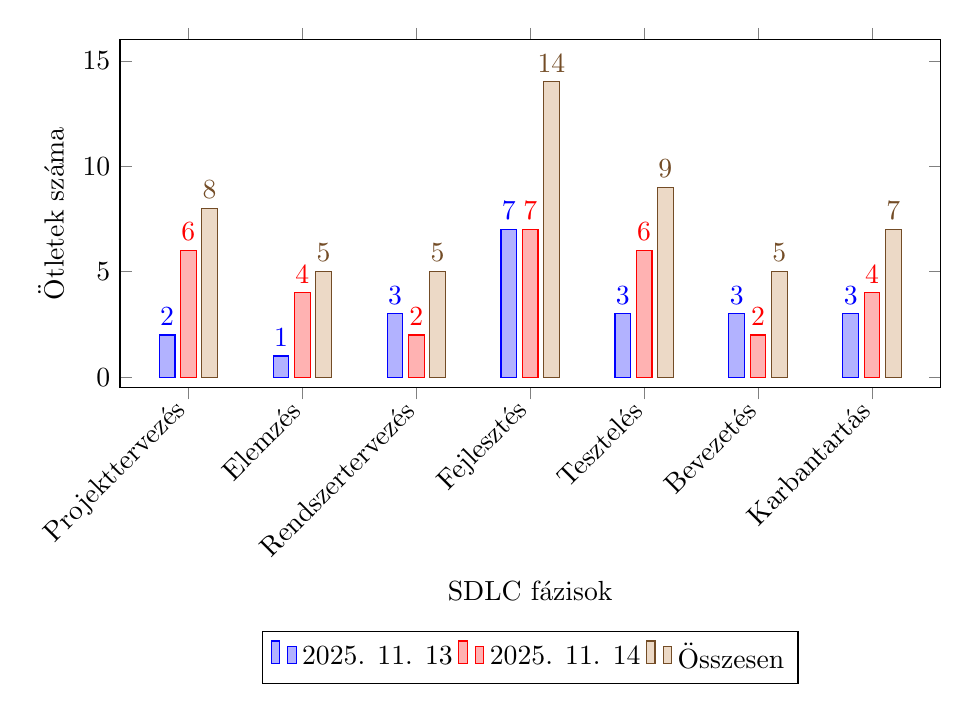
\begin{tikzpicture}
		\begin{axis}[
			xlabel={SDLC fázisok},
			ylabel={Ötletek száma},
			ybar,
			bar width=0.2cm,
			width=12cm,
			height=6cm,
			ymax=16,
			legend style={at={(0.5,-0.7)}, anchor=north, legend columns=3},
			xtick={1,2,3,4,5,6,7},
			xticklabels={Projekttervezés, Elemzés, Rendszertervezés, Fejlesztés, Tesztelés, Bevezetés, Karbantartás},
			x tick label style={rotate=45, anchor=east},
			ylabel near ticks,
			nodes near coords,
			]
			
			\addplot coordinates {(1,2) (2,1) (3,3) (4,7) (5,3) (6,3) (7,3)};
			\addlegendentry{2025. 11. 13}
			
			\addplot coordinates {(1,6) (2,4) (3,2) (4,7) (5,6) (6,2) (7,4)};
			\addlegendentry{2025. 11. 14}
			
			\addplot coordinates {(1,8) (2,5) (3,5) (4,14) (5,9) (6,5) (7,7)};
			\addlegendentry{Összesen}
		\end{axis}
	\end{tikzpicture}
	\caption{A panelbeszélgetéseken elhangzott ötletek eloszlása SDLC fázisok szerint. (Saját szerkesztés.)}
	\label{fig:sdlcbrainstorming}
\end{figure}

\subsection{Projekttervezés}

A projekttervezés során határozzuk meg a szoftverprojekt célját, hatókörét, erőforrásait és kockázatait. Másképp megfogalmazva meg kell határoznunk, hogy \textit{mit} (cél, hatókör) és \textit{mivel} (erőforrások, kockázatok) fogunk csinálni. Noha a szakirodalom kevés konkrét, valós felhasználási esetet említ ebből a fázisból, a megkérdezettek a jövőbe tekintő spekulációk mellett beszámoltak konkrét tapasztalatokról is, jóllehet, azok gyakran inkább még csak kísérletezésnek tekinthetők.

\paragraph{Helyzetfelmérés.}
A projekttervezés első lépése rendszerint az aktuális helyzet feltérképezése, amely egyaránt jelentheti a szervezet belső működését és a külső környezetet. A belső működés kapcsán fel kell mérni a használt folyamatokat, a meglévő rendszereket, azok főbb komponenseit, valamint a mindezek közt húzódó kapcsolatokat. A küldő környezetnek meghatározó elemei többek között a versenytársak és a szabályozók. Mindezekről rendszerint sokféle, töredezett, heterogén információ áll rendelkezésre, amelyek feldolgozása és összegzése időigényes emberi feladat. A GMI ugyanakkor hatékonyan képes feldolgozni és összefoglalni az ilyen széttagolt tudáshalmazokat.

A GMI ez irányú hatékony használatához elengedhetetlen a belső vállalati működést leíró dokumentumok beemelése a modell kontextusába. Mivel ezek általában érzékeny üzleti adatokat tartalmaznak, felmerülnek adatvédelmi aggályok az adatok sorsát illetően \parencite{CopilotingFuture}. Amennyiben az adatok nem oszthatók meg az MI modellel, az nagyban korlátozza a hatékonyságot. Megoldás lehet az is, ha egy vállalat saját maga futtat on-premise MI modellt, de ennek komoly hardverberuházási költsége van (a nagyméretű modellek futtatásához olyan nagy hardverkapacitásra van szükség, amelyet egyetlen vállalat reálisan nem tud hatékonyan kihasználni). Ennek alternatívája, amikor a modellek virtuális privát felhőben futnak, vagyis a hardvert nem kell megvásárolni, mégis biztonsági mechanizmusok gátolják meg a vállalati adatok kiszivárgását.

\paragraph{Brainstorming.} A projekttervezés potenciális eleme az ötletgyűjtés, vagyis a lehetséges fejlesztési irányok, megoldások, kiegészítő funkciók összegyűjtése. A brainstorming célja nem a mély technikai elemzés, hanem a lehetőségek minél sokszínűbb feltérképezése. A generatív MI ebben kifejezetten hatékony, hiszen képes a megadott célok és korlátok mentén nagyszámú ötletet és hivatkozást összegyűjteni.

Az ilyen típusú ötletgenerálás különösen hasznos akkor, amikor a projekt kezdeti szakaszában „vakfoltok” merülhetnek fel, illetve amikor a csapatnak nincs kellő kapacitása szisztematikus kutatásra. Fontos ugyanakkor kiemelni, hogy a GMI nem helyettesíti a mély domain-szakértelmet, inkább csak széleskörű, de gyakran felszínes irányokat tud mutatni, amelyek közül már az emberi tudás és intuíció alapján érdemes választani.

\paragraph{Értékelés.} Az ötletelést követően elengedhetetlen az egyes koncepciók részletes értékelése, vagyis annak vizsgálata, hogy az adott javaslat mennyire életképes, milyen előnyei és hátrányai vannak, illetve milyen hozzáadott értéket képvisel. Ebben a lépésben a GMI képes strukturált érveket generálni (pro-kontra listák), rámutatva ezáltal olyan szempontokra, amelyek a fejlesztőcsapat számára elsőre nem kézenfekvőek, különösen, ha a csapat összetétele nem fedi le az összes releváns szakterületet. A panelbeszélgetések résztvevői is megemlítették, hogy a modellek gyakran váratlan, de releváns szempontokat hoznak fel egy adott ötlettel kapcsolatban.

Az értékelés fontos része lehet a rendelkezésre álló adatokra épülő elemzés is, pl. hogy egy új funkciót valóban használna-e a felhasználói bázis. A GMI képes rövid szöveges összefoglalókat generálni nagy mennyiségű analitikai adatból és felhasználói visszajelzésből, ezzel hatékonyan támogatva a döntés-előkészítési folyamatot. Ennek a felhasználásnak természetesen előfeltétele, hogy megfelelő mennyiségű és minőségű adat áll rendelkezésre, amelyekből az MI modell dolgozni tud. Általánosságban is elmondható, hogy adat nélkül hatékony MI használat sincs.

\paragraph{Kockázatelemzés.} A projekttervezés során elengedhetetlen a kockázatok feltárása. A potenciális kockázatok tárháza szinte végtelen: technológiai, erőforrásbeli, üzemeltetési, biztonsági vagy megfelelőségi (compliance) kockázatokra egyaránt fel kell készülni. A GMI ebben a szakaszban jó kiegészítő eszköz lehet, hiszen rengeteg korábbi példát, iparági esetleírást, legjobb gyakorlatot (best practice) és dokumentációt használtak fel a modell tanítása során, amelyekből kiindulva képes lehet releváns kockázatokat azonosítani.

Az MI modellek ugyanakkor egyelőre nem helyettesíthetik a szakértők munkáját, hiszen csak a múltbeli példákból és az azokon felismert mintázatokból tud dolgozni, holott a kockázatok kimerítő feltárása a gyakorlatban gyakran igényel kreativitást. Ráadásul az adott szervezet egyedi kontextusát sem szabad figyelmen kívül hagyni, amely nem biztos, hogy kimerítően beemelhető a modell kontextusába. A GMI tehát ebben a szakaszban inkább a gondolkodási horizont szélesítésében, mintsem a döntéshozatalban játszik szerepet.

\paragraph{Becslés.} Egy projekt sikeressége többek között az idő- és erőforráskeretek betartásában mérhető, amelyek alapja a reális idő- és erőforrásbecslés. A generatív MI erre is használható: a modell a meglévő kódbázis, az érintett komponensek, korábbi hasonló projektek és fejlesztői becslések alapján képes előzetes idő- és munkaigénybecslést kalkulálni \parencite{GenAISWEresearchAgenda}. A panelbeszélgetések során is említették, hogy egy új funkció fejlesztéséhez szükséges időt a specifikáció és a forráskód fontosabb részei alapján a GMI modellek képesek meglepően pontosan megbecsülni.

\paragraph{Dokumentumgenerálás.} A projekttervezés végső kimenete általában formális dokumentum, mint pl. projektterv, kezdeti specifikáció, követelménylista, kockázatelemzés vagy becslési táblázat. A generatív MI jelentősen felgyorsíthatja ezeknek a dokumentumoknak az előállítását. A modell képes a rendelkezésre álló adatok, feljegyzések, részeredmények alapján jól strukturált, koherens  dokumentumokat generálni, amelyek és formai szempontból illeszkednek korábbi referenciamunkákhoz \parencite{Oracle2024_GenerativeAI_SoftwareDevelopment}.

A gyakorlatban ez nemcsak időt takarít meg, hanem javíthatja a dokumentumok minőségét is, mivel a modell képes konzisztens terminológiát, egységes szerkezetet és átlátható formátumot biztosítani. Ugyanakkor fontos látni, hogy a generált dokumentumokat minden esetben emberi utóellenőrzésnek kell alávetni, különösen tartalmi szempontból, hiszen a projekt további sikeressége szempontjából elengedhetetlen a pontosság garantálása.

\subsection{Elemzés}

Az elemzés során határozzuk meg és dokumentáljuk a szoftverrel szemben támasztott követelményeket. A követelmények célja, hogy a projekt minden résztvevője számára teljesen egyértelmű legyen, hogy a készítendő megoldásnak pontosan mire kell \textit{képesnek lennie} (funkcionális követelmények) és \textit{milyennek} kell lennie, vagyis milyen minőségi jellemzőkkel kell rendelkeznie a megoldásnak (extrafunkcionális követelmények). MI alapú követelményelemző eszközök léteznek ugyan a gyakorlatban is, de a GMI ilyen irányú felhasználása egyelőre inkább tűnik jövőbeli elképzelésnek, mint múltbeli gyakorlatnak.

\paragraph{Követelményszármaztatás.} A követelmények jelentős része származhat különböző dokumentumokból, amelyek tartalmát adottságként kell kezelni. Ezek egyaránt lehetnek belső vállalati (pl. illesztendő meglévő rendszerek tulajdonságai, belső információbiztonsági szabályzatok) és vállalaton kívüli (pl. szabályozói előírások – különösen szigorúan szabályozott nagyvállalati környezetben) források. A GMI képes lehet kinyerni ezekből a forrásokból a lényeges információkat, majd strukturálni és formális követelményekké alakítani azokat \parencite{rico2025challenges}, vagy pontosítani a már meglévő követelményeket, esetleg rámutatni hiányzó követelményekre. Az MI modell felismeri a követelményként értelmezhető mondatokat, és képes azokból egységes szerkezetű, pontos követelményeket származtatni. Ez különösen hasznos olyan projekteknél, ahol nagy mennyiségű kiinduló forrás tartalmaz potenciális követelményeket, ezek a források pedig heterogének, eltérő formátumúak.

Fontos ugyanakkor rámutatni, hogy egy szoftverprojekt szempontjából a követelmények összegyűjtése kritikus fontosságú. Ennek a fázisnak a precizitásán nagyban múlik a később szükséges iterációk száma, így az MI által származtatott követelményeket mindenképp szükséges emberi utóellenőrzés alá vetni. Kritikus fontosságú továbbá a követelmények teljességének az ellenőrzése, vagyis a megbizonyosodás arról, hogy valóban minden releváns követelmény összegyűjtésre került.

\paragraph{Követelményosztályozás.} A követelményeket általában osztályozzuk a jellegük szerint, vagyis az alapján, hogy mire vonatkoznak. Beszélhetünk funkcionális és extrafunkcionális követelményekről, utóbbi kategórián belül többek között teljesítményre, megbízhatóságra, biztonságra, megfigyelhetőségre, kompatibilitásra, karbantarthatóságra, használhatóságra vonatkozó követelmények. A GMI segíthet az elkészült követelmények osztályozásában \parencite{GenAISWEresearchAgenda}, ami elősegíti a rendezett követelménystruktúrát, és átláthatóbb dokumentációt eredményez.

\paragraph{Követelményminőség.} Bár a követelmények természetes nyelven kerülnek megfogalmazásra, a későbbiekben viszont egzaktan kell tudnunk ellenőrizni a megvalósulásukat, ezért kritikus fontosságú a precíz megfogalmazás. Ennek biztosítására különböző szabályok léteznek a megfogalmazására, amelyek célja a követelmények egyediségének, azonosíthatóságának, egyértelműségének és tesztelhetőségének biztosítása. Kerülni kell tehát a túl általános, homályos, félreérthető megfogalmazásokat, amelyekről nem dönthető el egyértelműen, hogy megvalósultak-e. A nagy nyelvi modellek képesek lehetnek ellenőrizni ezeket a megfogalmazásbeli elvárásokat, különösen, ha az elvárások minél részletesebben megfogalmazva állnak rendelkezésre.

\paragraph{Megvalósíthatóság.} A követelmények összegyűjtése után meg kell vizsgálni, hogy azok megvalósíthatók-e. A megvalósíthatóság több síkon is értelmezhető, mint pl. technikailag, üzletileg és erőforrások szempontjából. A megvalósíthatóság szükséges, de nem elégséges alapfeltétele a követelmények ellentmondás-mentessége. A generatív MI segíthet a potenciális ellentmondások, egymással nem összhangban lévő követelmények azonosításában, ami főleg nagy számú/terjedelmű követelmények esetében lehet különösen hasznos. A modellek akár képesek is lehetnek megoldási javaslatokat tenni az ellentmondások feloldására. Ugyanakkor az értelmezés és döntéshozatal továbbra is emberi feladat, hiszen a megvalósíthatóság végső megítélése mély szakterületi tudást igényel.

\subsection{Rendszertervezés}

A rendszertervezés során definiáljuk a rendszer logikai és technikai architektúráját, az adatmodelleket, valamint a komponensek közti kapcsolatokat és interfészeket. Gondos tervezéssel lehetséges az esetleges hibák korai feltárása, ami nagyban elősegíti a későbbi folyamatok (különösen a fejlesztés és a tesztelés), így összességében az egész SDLC hatékonyságát. A megkérdezettek tapasztalatai alapján a részletes rendszertervezést nem adják ki emberi kézből, de prototípusok generálására már most is aktívan használják a GMI-t.

\paragraph{Technológiaválasztás.} A technológiaválasztás során a fejlesztőcsapatnak meg kell határoznia, hogy a projekt mely eszközökre, keretrendszerekre, könyvtárakra és infrastruktúrára támaszkodik. Mivel vállalati környezetben a rendszerek jellemzően hosszútávra készülnek, a kiválasztás során nemcsak a jelen körülményeit kell figyelembe venni, hanem azt is, hogy a választott technológiák támogatása hosszútávon biztosított-e. Sőt, az is fontos mérlegelési szempont lehet, hogy mennyire közismert a technológia, hiszen ez közvetlenül befolyásolja, hogy mennyire könnyen (és milyen költségen) lehet fejlesztőt találni a projektre. A generatív MI képes lehet feltérképezni a potenciális megoldásokat (ideértve a \textit{state of the art}-ot is), összefoglalni a főbb előnyöket és hátrányokat, és mindezek alapján javaslatokat megfogalmazni \parencite{CopilotingFuture, rico2025challenges}. Ezek az ötletek segíthetnek ugyan a döntéshozók perspektívájának tágításában, de az MI modell javaslatainak kritikátlan felhasználása helyett nem szabad szem elől téveszteni a döntések súlyát, hiszen a technológiaválasztás hosszútávú következményekkel járhat az üzemeltetésre, a teljesítményre, a biztonságra és a bővíthetőségre nézve.

\paragraph{Prototipizálás.} A rendszertervezés fontos támogató tevékenysége a prototípusok készítése, amelyek célja a koncepciók gyors validálása és a magas szintű megoldási irányok gyakorlati kipróbálása. A generatív MI ebben a fázisban képes gyorsan létrehozni egyszerű proof-of-concept (PoC) vagy minimális életképes termék (minimal viable product, MVP) jellegű megoldásokat, beleértve az alapvető infrastruktúra-komponenseket vagy egyszerű felhasználói felületeket. Ez jelentős időmegtakarítást eredményezhet, különösen akkor, ha a projekt több lehetséges architektúrát is vizsgál, lehetővé téve azok összehasonlítását. Az összehasonlításon túl ez a módszer egy új technológia megismerésekor is hasznos lehet, hiszen egy egyszerű, ám mégis működő példán keresztül sokszor könnyebben elsajátítható az új tudás. Fontos azonban hangsúlyozni, hogy a prototípusokat a helyükön kell kezelni, azok semmiképp sem tekinthetők végleges terveknek. Az MI modellek által generált kód és architektúra sok esetben csak demonstrációs célokra alkalmas, és az sem garantált, hogy hűen reprezentálja az adott technológia használhatóságát.

\paragraph{Tervezés.} A GMI képes lehet egyszerűbb komponensek konkrét megtervezésére is, mint pl. egy egyszerű API (application programming interface, a szoftverkomponensek közti kommunikáció interfésze), valamint a vonatkozó metrikák (pl. szükséges tárhely, memória, sávszélesség) becslésében is segítséget nyújthat. Fontos azonban kiemelni, hogy még ha elsőre hívogatónak is tűnhet egy komplett rendszerterv legenerálása, valójában nagyon veszélyes. Egy komplex rendszerterv, különösen a hozzá kapcsolódó dokumentációk olyan összetettek és terjedelmesek, hogy azoknak a kellően tüzetes emberi utóellenőrzése egész egyszerűen irreális. A megkérdezettek ráadásul egyetértettek abban, hogy egy nem általuk készített komplex megoldás kellő részletességű átnézése valójában gyakran nehezebb és nagyobb szellemienergia-befektetést igényel, mint ha ők maguk készítették volna el, így pedig nagyon könnyű átsiklani az MI által vétett hibák felett.

\subsection{Fejlesztés}

A fejlesztés során ténylegesen implementáljuk a szoftvert, vagyis megvalósítjuk a rendszertervet. A megvalósításnak teljesítenie kell a korábban meghatározott követelményeket. Ebben a fázisban általában többnyire kódolás zajlik, amely eredményeként előáll a szoftver forráskódja. A GMI alkalmazása itt a legkézenfekvőbb és legelterjedtebb, amit több dolog is alátámaszt: egyrészt ehhez a fázishoz áll rendelkezésre a legtöbb GMI céleszköz, másrészt ezt (és a tesztelést) taglalja a legtöbb publikáció, harmadrészt a megkérdezetteknek is a kódolást illetően volt a legtöbb ötlete és tapasztalata.

\paragraph{Kódgenerálás.} A GMI kódgenerálásra (természetes nyelvi utasításokból programkód előállítása) való felhasználása jelentős időmegtakarítást eredményezhet, különösen a kevés tényleges gondolkodást igénylő, repetitív feladatok esetében. Ilyenek lehetnek többek között sablon (boilerplate) kódok, integrációs megoldások vagy a felhasználói felület (user interface, UI) egyszerű komponensei. A tapasztalatok szerint minél kevésbé komplex a feladat, annál hasznosabb a GMI, összetett üzleti logika vagy komplex technikai megoldások esetén viszont a modellek gyakran hibás vagy félrevezető kódot generálnak, és a javítás (vagy a modell rábírása a javításra) több erőfeszítést igényel, mint az önálló megírás \parencite{AI_pairprog, McKinseyDevProd, GenAITransformSWD}. A panelbeszélgetések résztvevői úgy foglalták össze ezt a jelenséget, hogy komplex esetekben hiába kezdik el lelkesen használni az MI-t a gondolkodás megspórolására, végül általában kiderül, hogy az \textit{igazán} bonyolult problémák végiggondolása, vagyis az \textit{igazi} gondolkodás nem spórolható meg.

A GMI-alapú kódgenerátorok alkalmazhatósága szempontjából kulcskérdés az adott szoftverkomponens szerepe: mivel a kódba kerülhetnek nehezen észrevehető hibák, a kevésbé fontos, nem kritikus részeken érdemes alkalmazni a technológiát. Azt is érdemes szem előtt tartani, hogy programnyelvenként eltérő garanciák vannak arra vonatkozóan, hogy milyen hibák milyen korán derülnek ki: míg egyes nyelvek lehet, hogy már le sem fordulnak, bizonyos szkriptnyelvek esetén elképzelhető, hogy csak jóval a bevezetés után, élesben derül majd fény egy hibára.

\paragraph{Megmagyarázás.} A generatív MI jól használható a meglévő kódrészek megértésének támogatására, ami különösen fontos nagy, rosszul dokumentált kódbázisok esetén. A modell képes összefoglalni, hogy egy adott függvény, osztály vagy modul mi célt szolgál, milyen bemeneteket és kimeneteket kezel, milyen kapcsolatban áll más komponensekkel, és mi a szerepe az egész rendszerben. Ez nagyban gyorsíthatja a fejlesztők munkáját, különösen új belépők vagy a projektbe frissen bekapcsolódó fejlesztők számára. A GMI megmagyarázó képessége újonnan írt kódok esetén is használható, többek között az új forráskód kommentezésével (kód ellátása magyarázó megjegyzésekkel) vagy a változások összefoglalásával (pl. verziókezelő számára).

\paragraph{Refaktorálás.} Refaktorálásnak nevezzük egy programkód átalakítását, a viselkedés módosítása nélkül, pusztán azért, hogy javuljon a kód struktúrája, olvashatósága, karbantarthatósága. A GMI hatékonyan támogathatja kisebb, jól körülhatárolt refaktorálási feladatok elvégzését, mint pl. változóátnevezés, kisebb logikai letisztázások, duplikációk eltávolítása, függvények szétbontása. Nagyobb léptékű, átfogó módosítások esetén azonban komoly kockázatot jelent, hogy a modell által generált változtatások olyan nagyok, hogy a fejlesztők már nem látják át teljesen, így végül vakon megbíznak az MI modellben. Ez magában hordozza a viselkedés akaratlan módosítását, ami olyan hibákat injektálhat a rendszerbe, amelyekre potenciálisan csak később, élesben derül fény. A megkérdezettek tapasztalatai is azt támasztották alá, hogy az MI által végzett refaktorálásokat mindenképp le kell ellenőrizni, mert könnyen végezhet nem várt, helytelen módosításokat is.

\paragraph{Hibakeresés.} A fejlesztési folyamat szerves részét képezi a készülő kód folyamatos kipróbálása és az iteratív hibakeresés, amelyben a generatív MI szintén nagy segítséget nyújthat. A modellek képesek értelmezni a kapott hibaüzeneteket, és a hibás kódban rámutatni a hibák tényleges okaira. A hibák szöveges magyarázatán túl képesek javaslatot tenni a javításra vagy akár konkrétan legenerálni a javított változatot. Ez még az egyszerű szintaktikai hibák esetén is hasznos lehet (pl. egy hosszú lekérdezésben könnyű apró hibákat véteni, amelyeket egyesével kijavítani jóval tovább tart, mint beadni az egészet az MI modellnek), de különösen hasznos, amikor a hiba valódi oka nem egyértelmű, egyszerűen csak egy váratlan viselkedésre keresünk magyarázatot.

\paragraph{Szkriptek.} A fejlesztés során gyakran adódnak olyan feladatok, amelyek nem tartoznak a fejlesztő szigorúan értelmezett szakterületéhez, de mégis meg kell őket oldania. Ez jelentheti akár bizonyos fejlesztői lépések automatizálását, akár adatok kinyerését fájlokból, a közös az bennük, hogy bár a feladatok egyszerűek, a praktikusan használt nyelvben (általában szkriptnyelv, pl. bash, awk) gyakran kevésbé magabiztos a fejlesztő, mert csak ritkán kényszerül használni. Ezek a feladatok tipikusan nem hordoznak jelentős kockázatot, és a generált megoldás is elég tömör és egyszerű ahhoz, hogy ,,ránézésre'' vagy első kipróbálásra megállapítható a helyessége, ugyanakkor jelentős időmegtakarítást eredményezhet, hogy nem kell egy kontextusváltás árán belemélyedni a ritkán használt nyelvbe. Bár nem szorosan tartozik ide, de mégis itt érdemes megemlíteni a reguláris kifejezések írását és értelmezését is, amiben szintén nagyon hasznos segítség lehet a GMI.

\paragraph{Konvertálás.} A fejlesztés során esetenként szükség van különböző fájlformátumok (pl. JSON, XML, CSV) közötti átalakításra, amit a GMI magabiztosan képes elvégezni. Az is előfordul, hogy egy adott programnyelven rendelkezésre álló logikát egy másik programnyelvben is elő kell állítani. Ez ugyan már jóval komplexebb feladat, mint egy fájlkonverzió, a tapasztalatok azt mutatják, hogy erre is használhatók a generatív MI modellek \parencite{GartnerAISWD, Oracle2024_GenerativeAI_SoftwareDevelopment}. A programnyelvek közti fordítás esetén is igaz, ami általánosságban is elmondható az MI által generált éles rendszerbe szánt kódokról: fontos megbizonyosodni a helyességről, akár emberi ellenőrzéssel, akár alapos teszteléssel.


\subsection{Tesztelés}

A tesztelés a szoftverfejlesztési életciklus kritikus fontosságú szakasza, melynek célja a szoftver minőségének biztosítása, a hibák feltárása, valamint annak igazolása, hogy az elkészült megoldás megfelel az előre meghatározott funkcionális és extrafunkcionális követelményeknek. A tesztelés hagyományosan erőforrásigényes és gyakran monoton tevékenység, amely azonban elengedhetetlen a későbbi, éles környezetben felmerülő, sokkal költségesebb hibák elkerülése érdekében. Mivel a tesztelés jelentős részét a tesztek megírása (kódolása) teszi ki, a fejlesztéshez hasonlóan itt is hatékony segítséget jelenthetnek a generatív MI megoldások. Ez a potenciál megmutatkozik a céleszközök és vonatkozó publikációk számában, és a megkérdezettek beszámolóiban is.

\paragraph{Tesztgenerálás.} A fejlesztők körében az egyik legnépszerűbb felhasználási mód a tesztek, különösen az egységtesztek (unit test) generálása (amely egy atomi funkcionális egység működését tesztelik). A GMI modellek képesek a forráskód alapján automatikusan teszteseteket írni, lefedve számos bemeneti kombinációt és végrehajtási ágat \parencite{PwC2024_GenAI_SWD_Improve, GenAITransformSWD}. Ez jelentősen növelheti a kódlefedettséget és csökkentheti a tesztírásra fordított időt.

Ugyanakkor fontos tisztában lenni egy súlyos módszertani korláttal: ha a teszteket a forráskódból származtatjuk (különösen, ha ugyanazzal a GMI modellel generáljuk őket, amely a forráskódot is generálta), az valójában \textit{fehér dobozos} tesztelést (white box testing) eredményez, ahol a tesztkészlet a kód belső működését tükrözi, nem pedig a specifikációt. Ha a kód hibás logikát vagy struktúrát tartalmaz, a generált tesztkészlet potenciálisan ehhez a hibás logikához fog illeszkedni, így hiába fut le sikeresen egy teszt, a tesztelni kívánt, de valójában nem tesztelt hiba mégis rejtve marad. A valódi minőségbiztosításhoz elengedhetetlen, hogy a tesztek a kódtól függetlenül, az elvárások (követelmények) alapján (is) készüljenek (\textit{fekete dobozos} tesztelés, black box testing).

\paragraph{Tesztadat-generálás.} A tesztelés során gyakori probléma a megfelelő minőségű és mennyiségű tesztadat előállítása. A valós éles adatok használata szigorú adatvédelmi és biztonsági kockázatokat vet fel, a kézi adatgyártás pedig lassú és nem skálázható. A generatív MI képes szintetikus, de a valós adatok statisztikai jellemzőit és struktúráját hűen tükröző tesztadatokat előállítani \parencite{PwC2024_GenAI_SWD_Improve}. Ez lehetővé teszi a fejlesztők számára, hogy biztonságosan teszteljenek határértékeket, kivételes eseteket vagy nagy adathalmazokat igénylő teljesítményteszteket végezzenek. Korlátot jelenthet ugyanakkor, hogy a generálás nem feltétlenül szisztematikus: a modell tanult minták alapján dolgozik, nem pedig algoritmikusan, így előfordulhat, hogy bizonyos speciális, de kritikus adatkombinációkat magától nem állít elő, hacsak a promptban erre külön nem utasítjuk.

\paragraph{Integrációs tesztelés.} Míg a unit tesztek a kód legkisebb funkcionális egységeit vizsgálják, az integrációs tesztelés a komponensek közötti együttműködés ellenőrzésére szolgál. Ez a terület komplexebb, mivel gyakran külső függőségeket, adatbázisokat vagy hálózati kommunikációt igényel. A fejlettebb, agentikus MI megoldások képesek lehetnek arra, hogy autonóm módon elindítsák a szükséges kódokat, felépítsék a tesztkörnyezetet, és szkriptek segítségével szimulálják és ellenőrizzék a komponensek közötti interakciókat \parencite{PwC2024_GenAI_SWD_Improve}. A GMI segíthet a komponenseket összekötő „ragasztó” kódok (glue code) és a teszteléshez szükséges konfigurációk elkészítésében is, ami jelentős terhet vesz le a tesztautomatizáló mérnökök válláról.

\paragraph{Kimenetellenőrzés.} A regressziós tesztelés során -- amikor azt vizsgáljuk, hogy egy módosítás nem rontott-e el korábban már működő funkciókat -- gyakran keletkeznek nagyméretű naplófájlok (logok) és kimeneti állományok. Ezek manuális átnézése rendkívül időigényes és az emberi figyelmet próbára tevő feladat. A generatív MI modellek hatékonyan használhatók a tesztfutások eredményeinek összehasonlítására. A modell képes összevetni az elvárt és a kapott kimenetet, kiemelni az eltéréseket, sőt, a hibaüzenetek alapján akár előzetes diagnózist is felállíthat a hiba lehetséges okáról, felgyorsítva ezzel a hibajavítási ciklust.

\paragraph{Kompatibilitásellenőrzés.} A szoftverek fejlődésének természetes velejárója a változás, azonban bizonyos helyzetekben fontos szempont a visszafelé kompatibilitás (backward compatibility) biztosítása, különösen API-k vagy mások (akár szervezete belül, akár azon kívül) által is használt könyvtárak esetén. A generatív MI segíthet a tervezett változtatások elemzésében, összevetve a régi és az új verzió interfészét és belső működését. A modell képes azonosítani azokat a módosításokat (pl. egy függvény szignatúrájának megváltozását vagy a belső működés nem kívánt megváltozását), amelyek problémát okozhatnának a szoftvert használóknál, még azelőtt, hogy a módosítás éles környezetbe kerülne.

\paragraph{Kódátvizsgálás.} A kódátvizsgálás (code review) kettős szerepet tölt be a GMI kontextusában. Egyrészt az ember által írt kód MI általi ellenőrzése értékes eszköz: a modellek \textit{fáradhatatlanul} képesek kiszűrni a szintaktikai hibákat, a biztonsági sérülékenységeket, vagy javaslatokat tenni a kód stílusának javítására \parencite{Oracle2024_GenerativeAI_SoftwareDevelopment, PwC2024_GenAI_SWD_Improve, GenAITransformSWD}, míg emberi ellenőrzés esetén számolni kellene a figyelem lankadásának veszélyével.

Másrészt viszont komoly kihívást jelent az MI által generált kód emberi felülvizsgálata. A kutatások és a gyakorlati tapasztalatok azt mutatják, hogy ha a kódot nagyrészt az MI generálja, az emberi fejlesztő hajlamos a felületes ellenőrzésre. Egyrészt pszichológiailag nehezebb és unalmasabb más (vagy egy gép) kódját olvasni és értelmezni, mint sajátot írni. Másrészt az MI által generált kód szintaktikailag általában helyes és „szépnek” tűnik, ami hamis biztonságérzetet ad. Így a fejlesztők könnyen átsiklanak olyan logikai vagy szemantikai hibák felett, amelyeket saját kódolás közben nem vétettek volna el, vagy azonnal észrevettek volna. Paradox módon tehát az MI által generált kód ellenőrzése esetenként nagyobb kognitív terhelést és fegyelmet igényel, mint a kódolás maga.

\subsection{Bevezetés}

A bevezetés fázis képez hidat a fejlesztés és az üzemeltetés között, amely során az elkészült szoftver kikerül a védett, elszeparált fejlesztői környezetből és élesben elérhetővé válik a végfelhasználók számára. Ez a szakasz különösen kritikus, hiszen bármilyen hiba közvetlen hatással van a szolgáltatás elérhetőségére és az \textit{üzletmenet folytonosságára}. Bizonyára ezzel is magyarázható, hogy ebben a fázisban a GMI használata egyelőre inkább csak spekulációnak tűnik, valós ipari tapasztalatok nemigen állnak rendelkezésre.

\paragraph{Infrastruktúrakód.} A modern felhőalapú környezetekben az infrastruktúra kezelése már nem manuális kattintgatással, hanem kód formájában történik (Infrastructure as Code, IaC). A generatív MI modellek képesek legenerálni vagy módosítani ezeket a deklaratív konfigurációs fájlokat. Mivel ezek a leíró nyelvek szigorú struktúrával rendelkeznek, az MI képes a természetes nyelven megfogalmazott igényeket szintaktikailag helyes konfigurációs kóddá alakítani.

\paragraph{Függőségelemzés.} A bevezetés előtt álló szoftvercsomagok gyakran tartalmaznak külső könyvtárakat és modulokat. A generatív MI segíthet a függőségek (dependency) elemzésében, feltárva az esetleges verzióütközéseket vagy ismert biztonsági sérülékenységeket. Ez azért lehet különösen hasznos, mert ezek a hibák gyakran akár hosszú ideig is rejtve maradhatnak, és csak később, éles futás közben, váratlanul okoznak problémát.

\paragraph{Dokumentáció.} A bevezetés elengedhetetlen része a változások dokumentálása (enélkül ugyanis többek között elképzelhetetlen a hatékony változásmenedzsment). A fejlesztés és tesztelés során keletkező technikai információkból (commit üzenetek, hibajegy, CI/CD logok) a generatív MI képes meghatározott célú dokumentációt generálni. Ez egyaránt jelentheti a fejlesztőknek és üzemeltetőknek szóló technikai leírásokat, vagy a végfelhasználóknak szánt közérthető verzióinformációkat (release notes) és felhasználói kézikönyveket \parencite{PwC2024_GenAI_SWD_Improve}. Ez azért is lehet hiánypótló a gyakorlatban, mert a fejlesztők általában nem szívesen, csak muszájból írnak dokumentációt, így annak a mennyisége, minősége és naprakészsége gyakran nem kielégítő.

\paragraph{Végrehajtás.} Az autonóm ágensek megjelenésével megnyílt a lehetőség arra, hogy az MI hajtsa is végre a telepítési folyamatot. Ez azonban rendkívüli kockázatot hordoz: ahhoz, hogy egy ágens telepíteni tudjon, írási hozzáférést kell kapnia az éles (production) környezethez. Mivel a nagy nyelvi modellek működése nem determinisztikus, a közvetlen hozzáférés katasztrofális következményekkel járhat. Ezt támasztja alá az a közelmúltbeli eset is, amikor egy MI alapú kódoló eszköz véletlenül törölte egy vállalat éles adatbázisát, majd kérdésre „letagadta”, és azt állította, hogy nem történt törlés \parencite{Replit_Database_Delete_2025}. Az eset rávilágít arra, hogy az emberi felügyelet nélküli közvetlen hozzáférés az éles környezethez jelenleg elfogadhatatlan kockázatot jelent.

\paragraph{Folyamat definiáltsága.} A bevezetéssel kapcsolatban kirajzolódik egy érdekes paradoxon a generatív MI szerepét illetően. A sikeres automatizáció kulcsa a folyamat pontos definiálása. Ha egy szervezetnél a telepítési folyamat nincs pontosan definiálva (ad-hoc jellegű), akkor az MI ágens sem fogja tudni sikeresen végrehajtani, hiszen hiányzik a kontextus és a szabályrendszer. Ha viszont a folyamat lépései (pipeline) precízen, egzaktan definiálva vannak, akkor azok leprogramozhatók hagyományos, determinisztikus eszközökkel (szkriptek, CI/CD eszközök), amelyek utána 100\%-os megbízhatósággal működnek. Ebben az esetben a nemdeterminisztikus, potenciálisan hibázó GMI használata a végrehajtásra felesleges kockázatot visz a rendszerbe. A GMI helye tehát nem a folyamat \textit{futtatásában}, hanem a folyamatot leíró automatizációs kódok \textit{létrehozásában} van.


\subsection{Karbantartás}

A szoftverek életciklusa nem ér véget a sikeres bevezetéssel, az ezt követő karbantartási fázis időben gyakran a leghosszabb az összes fázis közül, hiszen különösen nagyvállalati környezetben a szoftverek gyakran évtizedekig üzemelnek. Ebben a fázisban a cél a rendszer stabil működésének biztosítása, a felhasználók támogatása, az esetlegesen felmerülő hibák javítása, valamint a potenciális továbbfejlesztési igények kezelése. A GMI vonatkozó felhasználása értelemszerű lenne, de többségében egyelőre mégis inkább csak vágyálom -- kivéve az ügyféltámogatást, hiszen ilyen chatbotokkal már bizonyára mindenki találkozott.

\paragraph{Hibajegy-előfeldolgozás.} Az üzemeltetés során beérkező hibajegyek (ticket) kezelése jelentős emberi erőforrást igényel, különösen azért, mert a bejelentések gyakran pontatlanok, hiányosak vagy duplikáltak. A generatív MI képes a beérkező természetes nyelvű bejelentések előfeldolgozására: osztályozza a hibákat súlyosság és típus szerint, valamint összeveti azokat más esetekkel, hogy azonosítsa az ismétlődéseket. Amennyiben a bejelentésből hiányoznak nélkülözhetetlen adatok, a modell automatikusan bekérheti ezeket a bejelentőtől még azelőtt, hogy a jegy egy fejlesztőhöz kerülne. Ezen felül az MI képes lehet egy hibajegy szempontjából releváns naplófájlok beazonosítására is, sőt, megfelelő jogosultságokkal akár közvetlenül csatolhatja is azokat a hibajegyhez.

\paragraph{Hibaokfeltárás.} Egy hiba részletes kivizsgálása, különösen a tényleges kiváltó ok megtalálása gyakran nehéz fejlesztői feladat, hiszen nagy mennyiségű információ (forráskód, naplófájlok, stack trace, hibajegy) között kell megtalálni az összefüggéseket. A generatív MI modellek hatékonyan támogatják a kiváltóok-elemzést (root cause analysis, RCA): a rendelkezésre álló információk alapján képesek hipotéziseket felállítani a hiba lehetséges okairól \parencite{Oracle2024_GenerativeAI_SoftwareDevelopment, PwC2024_GenAI_SWD_Improve}. Bár a modell által javasolt diagnózis nem minden esetben pontos, mégis gyakran jelent hasznos kiindulási pontot, csökkentve ezzel a hiba kijavításához szükséges időráfordítást.

\paragraph{Teljesítményelemzés.} A karbantartás nemcsak a hibajavításról, hanem a rendszer hatékonyságának fenntartásáról is szól. A rendszerekbe az élettartamuk során jellemzően egyre több adat kerül, aminek a hatékony kezelése pl. skálázódási kihívásokat jelenthet a későbbiekben. A generatív MI segíthet a teljesítménybeli szűk keresztmetszetek (bottleneck) azonosításában. A kód statikus elemzésével vagy a futásidejű profilozási adatok értelmezésével a modell rámutathat azokra a kódrészletekre (pl. nem hatékony adatbázis-lekérdezések, felesleges fájlműveletek, cache-elés hiánya), amelyek lassítják a rendszer működését, és optimalizációs javaslatokat tehet azok javítására.

\paragraph{Ügyféltámogatás.} A generatív MI egyik leglátványosabb felhasználási területe a felhasználókkal való közvetlen kapcsolattartás. A nagy nyelvi modellekre épülő chatbotok képesek intelligens ügyfélszolgálati (customer service) feladatokat ellátni, válaszolva a gyakori kérdésekre vagy segítve a felhasználókat a szoftver használatában \parencite{GartnerGenAI4Enterprise}. Ez tehermentesíti az emberi ügyfélszolgálatot, akik így a komplexebb problémákra fókuszálhatnak. Emellett a GMI felhasználható a felhasználói visszajelzések (feedback) elemzésére és összegzésére is, segítve a termékmenedzsereket abban, hogy a nagy mennyiségű szöveges értékelésből kiszűrjék a leggyakoribb igényeket és panaszokat. Fontos azonban a kockázatok szem előtt tartása és kezelése: a közvetlen ügyfélkommunikációban az MI tévedései (pl. hallucináció) reputációs károkat okozhat.

\chapter{Következtetések}\label{ch:kovetkeztetesek}

Ebben a fejezetben kutatási eredményeim összefoglalásául következtetéseket fogalmazok meg: az \ref{sec:kovetkeztetes-megiteles}. alfejezetben a generatív mesterséges intelligencia megítélését illetően, az \ref{sec:kovetkeztetes-szerep}. alfejezetben a technológia szerepéről és lehetséges felhasználásairól, az \ref{sec:kovetkeztetes-kihivasok}. alfejezetben a kapcsolódó kihívások és tapasztalatok vonatkozásában. Az \ref{sec:akciolista}. alfejezetben bemutatok egy akciólistát a generatív MI sikeres bevezetéséhez, végül az \ref{sec:kutmod-ertekeles}. alfejezetben értékelem az alkalmazott kutatásmódszertant.

\section{A generatív mesterséges intelligencia megítélése}\label{sec:kovetkeztetes-megiteles}

A kutatás során kirajzolódott kép alapján a szoftverfejlesztők a generatív mesterséges intelligenciára (GMI) alapvetően mint egy nagy tudású, univerzális, fáradhatatlan, ám korántsem tévedhetetlen asszisztensre tekintenek. A technológia megítélése kettős: miközben elismerik a benne rejlő kényelmet és potenciált, a szakemberek tisztán látják annak (jelenlegi) korlátait is.

\paragraph{Univerzális.} A GMI lett a modern szoftverfejlesztés kalapácsa: \textit{akinek kalapács van a kezében, az hajlamos mindent szögnek nézni} \parencite{maslow1966psychology}. Mivel a nagy nyelvi modellek univerzálisak és rendkívül kényelmesen használhatók természetes nyelven, a fejlesztők hajlamosak olyan feladatokra is ezt használni, amelyekre léteznek pontosabb, megbízhatóbb céleszközök. A GMI „mindenhez ért”, de speciális technikai feladatokban (pl. statikus kódanalízis, refaktorálás) gyakran elmarad a determinisztikus algoritmusok pontosságától. A gyakorlatban a kényelem azonban sokszor felülírja a racionalitást, ami kockázatot jelent.

\paragraph{Absztrahálás hiánya.} A megkérdezettek szerint a generatív MI jelenlegi formájában nem képes az emberi gondolkodás egyik legfontosabb elemére, az \textit{absztrahálásra}. Mivel a modellek a meglévő adatokon, a múltban keletkezett mintázatokon tanulnak, működésükből hiányzik a valódi kreativitás, az igazi „out of the box” gondolkodás. A szoftverfejlesztés lényege gyakran éppen az egyedi, korábban nem látott (üzleti) problémák leképezése absztrakt modellekre, amit a jelenlegi GMI eszközök önállóan nem tudnak elvégezni. Így pedig a szoftverfejlesztés legértékesebb és legfárasztóbb része, azaz a problémák \textit{megértése} és az \textit{„igazi” gondolkodás} továbbra sem spórolhatók meg.

\paragraph{Megbízhatóság.} A technológia megítélését negatívan befolyásolják a megbízhatósági problémák, különösen a hallucináció jelensége. A fejlesztők számára frusztráló, hogy az eszközök gyakran magabiztos stílusban közölnek teljesen téves információkat. Szintén negatív jelenségként értékelhető a tartalom felesleges felduzzasztása. Abszurd helyzeteket teremt, amikor az egyik MI modell által generált, információban ritka, de terjedelmes szöveget egy másik modellel kell összefoglaltatni a hatékony feldolgozáshoz. Ez rávilágít arra, hogy a technológia jelenleg a redundáns emberi kommunikációt utánozza, ahelyett, hogy a szoftverfejlesztésben elvárt precizitást és tömörséget célozná meg.

\paragraph{Munkaerőpiac.} A munkaerőpiaci kilátásokat illetően a kutatás nem igazolta vissza a fejlesztők munkájának megszűnésével kapcsolatos félelmeket. A megkérdezettek nem féltik a munkájukat, sőt, egyetértés mutatkozik abban, hogy a jövőben is szükség lesz olyan szakemberekre, akik képesek a valós világ problémáit digitális megoldásokra fordítani. Ehhez ugyanis mindkét világ – az üzleti domain és a technológia – mélyreható ismerete szükséges. A következtetés szerint a szoftverfejlesztő munkakör átalakul, de nem szűnik meg: az MI nem kiváltja az embert, hanem a segítőjévé válik a mindennapi munkában.

\paragraph{Kilátások.} Végezetül megállapítható, hogy a technológia megítélése széles skálán mozog attól függően, hogy az egyén mennyire mélyedt el a használatában. Arról azonban ettől függetlenül majdhogynem egyetértés uralkodik, hogy a technológiát övező várakozások gyakran inkább a fantázia, semmint a tapasztalatok szüleményei.

\section{A generatív mesterséges intelligencia szerepe}\label{sec:kovetkeztetes-szerep}

Kutatásom alapján a generatív mesterséges intelligencia a szoftverfejlesztési életciklus (SDLC) számos pontján képes értéket teremteni, azonban a jelenlegi felhasználás eloszlása egyenletlen. A GMI felhasználásának szempontjait az \ref{tab:szempontok}. táblázat tartalmazza.

\begin{table}[htbp]
	\centering
	\caption{A GMI felhasználásának szempontjai. (Saját szerkesztés.)}
	\label{tab:szempontok}
	\begin{tabular}{p{3cm} p{5cm} p{5cm}}
		\toprule
		\textbf{Szempont} & \textbf{Pozitív} & \textbf{Negatív} \\
		\midrule
		\textbf{Felhasználási terület} & Fejlesztésben, tesztelésben hatékony segítség & Többi SDLC fázisba még nincs megfelelően integrálva\\
		\midrule
		\textbf{Hibatűrés} & Könnyen javítható dolgokra alkalmas & Kritikus feladatokra kockázatos \\
		\midrule
		\textbf{Felhasználási mód} & Ellenőrzésre kiváló & Generálás eredményét nehéz utóellenőrizni \\
		\midrule
		\textbf{Kezdeti tapasztalatok} & 5\% siker & 95\% kudarc \\
		\bottomrule
	\end{tabular}
\end{table}

\paragraph{Felhasználási terület.} A legszembetűnőbb következtetés a kódolási és tesztelési fázisok túlreprezentáltsága. Mind a szakirodalmi áttekintés, mind a panelbeszélgetések tapasztalatai azt mutatják, hogy a fejlesztők és az eszközgyártók fókusza elsősorban a kódgenerálásra irányul. Itt áll rendelkezésre a legtöbb tapasztalat, ezzel szemben az SDLC többi fázisában inkább csak kísérletezés zajlik. Ez egyben rámutat egy kihasználatlan potenciálra is: a valódi hatékonyságnöveléshez a generatív MI-t a teljes életciklusban alkalmazni kellene, nem csak a fejlesztési idő kisebb részét kitevő kódolásban \parencite{gartner_ai_sdlc}.

A \ref{ch:eredmenyek}. fejezetben bemutatott felhasználási lehetőségeket a \textit{Kísérletezés/Spekuláció}, \textit{Kezdeti tapasztalatok} és \textit{Aktív használat} kategóriákba soroltam, amit a \ref{tab:felhasznalasok}. táblázat tartalmaz. A besorolás nem reprezentatív (hiszen elsősorban a panelbeszélgetéseken alapul, mivel a szakirodalomban bemutatott lehetőségekről gyakran nem állapítható meg, mennyire tartoznak hozzájuk valós ipari felhasználások is), de ennek ellenére is jó áttekintést ad az eredményeimről.

\begin{table}[htbp]
	\centering
	\caption{A GMI használati lehetőségeinek besorolása SDLC fázisok és elterjedtség szerint. (Saját szerkesztés.)}
	\label{tab:felhasznalasok}
	\begin{tabular}{p{2.5cm} p{4.2cm} p{3.8cm} p{3cm}}
		\toprule
		\textbf{SDLC fázis} & \textbf{Kísérletezés\slash Spekuláció} & \textbf{Kezdeti\newline tapasztalatok} & \textbf{Aktív használat} \\
		\midrule
		\textbf{Projekt\-tervezés} & Helyzetfelmérés\newline Brainstorming\newline Értékelés\newline Kockázatelemzés & Dokumentum\-generálás\newline Becslés & \\
		\midrule
		\textbf{Elemzés} & Követelmény\-származtatás\newline Követelmény\-osztályozás\newline Követelményminőség\newline Megvalósíthatóság & & \\
		\midrule
		\textbf{Rendszer\-tervezés} & Tervezés & Technológia\-választás\newline Prototipizálás & \\
		\midrule
		\textbf{Fejlesztés} & & & Kódgenerálás\newline Megmagyarázás\newline Refaktorálás\newline Hibakeresés\newline Szkriptek\newline Konvertálás \\
		\midrule
		\textbf{Tesztelés} & Kimenetellenőrzés\newline Kompatibilitás\-ellenőrzés & Integrációs tesztelés & Tesztgenerálás\newline Tesztadat-generálás\newline Kódátvizsgálás \\
		\midrule
		\textbf{Bevezetés} & Infrastruktúrakód\newline Függőségelemzés\newline Végrehajtás & Dokumentáció & \\
		\midrule
		\textbf{Karbantartás} & Hibajegy-előfeldolgozás\newline Teljesítményelemzés & Hibaokfeltárás & Ügyféltámogatás \\
		\bottomrule
	\end{tabular}
\end{table}

\paragraph{Hibatűrés.} A GMI szerepének meghatározásakor kulcskérdés a feladat kritikussága és a hibatűrés mértéke. A technológia kiválóan alkalmazható olyan területeken, ahol a hiba megengedhető, mert „olcsó” vagy könnyen javítható (pl. prototípus készítése, egy UI elem stílusának generálása), de kockázatos a kritikus rendszerek (pl. közlekedés, energetika, pénzügy) esetében. A következtetés az, hogy a GMI szerepe a kockázatmentes kísérletezés és a gyors prototipizálás területén a legjelentősebb, míg az éles, biztonságkritikus rendszerekben a szerepe korlátozottabb kell, hogy maradjon.

\paragraph{Felhasználási mód.} Kutatásom rávilágított egy fontos emberi aspektusra a tartalomlétrehozás kapcsán. Bár a GMI képes nagy mennyiségű kódot vagy dokumentációt generálni, az emberi természetből fakadó lustaság miatt fennáll a veszélye, hogy ezeket a kimeneteket a felelős személyek nem ellenőrzik megfelelő alapossággal. Ezzel szemben a technológia sokkal biztonságosabban használható az ellenkező irányban: ember által írt kódok vagy szövegek ellenőrzésére (review), kontextus magyarázatára vagy hibakeresésre. Ebben az esetben az MI „fáradhatatlan” figyelme kiegészíti az emberi kreativitást.

\paragraph{Kezdeti tapasztalatok.} Végezetül fontos következtetés, hogy a GMI vállalati integrációja jelenleg gyerekcipőben jár. Ahogy arra az MIT friss kutatása is rámutatott, a projektek jelentős része, akár 95\%-a kudarcot vall vagy nem hoz átütő sikert, mert a megoldások szigetszerűek maradnak \parencite{NANDA2025_GenAIDivide}. A technológia nem illeszkedik szervesen a meglévő vállalati folyamatokba, nem éri el a belső tudásbázisokat. Ez arra enged következtetni, hogy a GMI sikeres alkalmazása ma már nem elsősorban technológiai, hanem vezetési, szervezési és folyamatmenedzsment kihívás.

\section{A generatív mesterséges intelligencia használatának kihívásai}\label{sec:kovetkeztetes-kihivasok}

A kutatási eredmények alapján a generatív MI szoftverfejlesztésbeli alkalmazását számos, nem tisztán technológiai kihívás nehezíti. Ezek a gátló tényezők gyakran erősebbnek bizonyulnak, mint maga a technológiai korlát. A GMI használatának főbb kihívásait az \ref{tab:kihivasok}. táblázat tartalmazza.

\begin{table}[htbp]
	\centering
	\caption{A GMI használatának főbb kihívásai. (Saját szerkesztés.)}
	\label{tab:kihivasok}
	\begin{tabular}{p{2.2cm} p{3.5cm} p{3.7cm} p{3.5cm}}
		\toprule
		\textbf{Szint} & \textbf{Kihívás}                   & \textbf{Adottság}       & \textbf{Kulcsszavak}                   \\
		\midrule
		Ország         & Jogi környezet                     & Jogszabályok            & Törvény\newline Compliance                    \\
		\midrule
		Szervezet      & Vállalati környezet                & Belső szabályok         & Policy\newline Compliance                     \\
		\midrule
		Szervezet      & Tudásintegráció                    & Szervezeti tudás        & Heterogén\newline Fragmentált       \\
		\midrule
		Ember          & Emberi tényezők\newline és kompetenciák  & Személyes tudás         & Prompt engineering\newline Deskilling         \\
		\midrule
		Ember          & Pszichológiai csapda               & Emberi természet        & Utóellenőrzés\newline Unalom                  \\
		\midrule
		Technológia    & Műszaki korlátok\newline és költségek    & Technológiai fejlettség & Nemdeterminizmus\newline Hallucináció\newline Token \\
		\bottomrule
	\end{tabular}
\end{table}

\paragraph{Jogi és vállalati környezet.} A nagyvállalati környezetben a legfőbb akadályt a jogi bizonytalanság és az adatbiztonsági szigor jelenti. A cégek érthető módon védik szellemi tulajdonukat és ügyféladataikat, ami szélsőséges esetben ahhoz vezet, hogy a biztonsági megoldások gyakorlatilag kiüresítik az MI eszközöket, feláldozva a potenciális hatékonyságnövelést. A fejlesztők így sokszor nem a legmodernebb eszközökhöz férnek hozzá, vagy ha igen, akkor nem tudják azokat a releváns adatokkal és rendszerekkel használni.

\paragraph{Tudásintegráció.} A GMI hatékony működésének feltétele a kontextus ismerete. Egy szoftverfejlesztési projekt tudásanyaga azonban széttöredezett: a követelmények és dokumentumok, a kód és az adatok mind más rendszerben vagy adatbázisban találhatók. Ezen heterogén források biztonságos és naprakész integrálása a nyelvi modellek kontextusába komoly architekturális kihívás, ám enélkül a modell csak általános válaszokat tud adni, nem pedig specifikus segítséget.

\paragraph{Emberi tényezők és kompetenciák.} A technológia használata új kompetenciákat igényel, mint például a \textit{prompt engineering}. Ez nem csupán technikai tudás, hanem egy újfajta kommunikációs készség, amelyet tanulni kell. A szervezeteknek időt és teret kell biztosítaniuk ennek elsajátítására. Ugyanakkor felmerül az „elbutulás” (deskilling) kockázata is: ha a fejlesztők túlságosan hozzászoknak az MI segítségéhez, elveszíthetik rutinjukat az alapszintű problémamegoldásban, és előfordulhat, hogy MI támogatás nélkül már nem lesznek képesek hatékonyan dolgozni \parencite{CopilotingFuture}.

\paragraph{Pszichológiai csapda.} A szoftverfejlesztésben az MI ígérete az, hogy átveszi az unalmas, repetitív munkát. Ezzel azonban egy új, még unalmasabb feladatot teremt: a generált kimenetek átnézését és validálását. Az emberi természetből fakadóan a monoton ellenőrzési feladatok során lankad a figyelem. Ez a helyzet veszélyes hibákhoz vezethet: a fejlesztők hajlamosak átsiklani olyan MI által generált hibák felett, amelyeket ők maguk talán el sem követtek volna, vagy saját kódolás közben azonnal észrevettek volna.

\paragraph{Műszaki korlátok és költségek.} A modellek használata nem ingyenes; a tokenek (számítási egységek) fogyása közvetlen költséget jelent, melyet menedzselni kell. Emellett technikai kihívást jelent a reprodukálhatóság hiánya: a nemdeterminisztikus modellek ugyanarra a bemenetre eltérő kimenetet adhatnak, ami megnehezíti a tesztelést és a validálást \parencite{LLMthreats}. A hallucináció kiküszöbölésére megoldást jelenthetne az LLM válaszok automatizált validálása, ehhez azonban szükség lenne a validálandó tudás formalizálására, hiszen jelenleg a tudás természetes nyelven áll rendelkezésre, nem pedig matematikai formalizmusok által leírva.

\section{Akciólista a generatív mesterséges intelligencia bevezetéséhez}\label{sec:akciolista}

A kutatási eredmények és a feltárt kihívások alapján az alábbi lépésekből álló akciótervet javaslom a technológia sikeres szervezeti bevezetéséhez:

\begin{enumerate}
	\item \textbf{Jogi és szabályozási környezet tisztázása.} Az első és legfontosabb lépés egy világos, mindenki számára elérhető szabályrendszer megalkotása. A fejlesztőknek tudniuk kell, mely eszközöket használhatják, milyen adatokat oszthatnak meg ezekkel, és hol húzódnak a tilalmak határai. A bizonytalanság megszüntetése kulcsfontosságú a technológia használatának széleskörű elterjedéséhez.
	
	\item \textbf{Mérhető keretrendszer kialakítása.} A bevezetés sikerességének nyomon követéséhez mérőszámokra van szükség. Definiálni kell, mit tekintünk sikernek (pl. fejlesztési ciklusidő csökkenése, hibák számának csökkenése), és mérni kell a ráfordításokat is (pl. licenszköltségek, tokenhasználat). A megtérülés (return of investment, ROI) nyomon követése segíti a tisztánlátást, és alapot ad a technológia skálázását illető döntések előkészítéséhez.
	
	\item \textbf{Vállalati tudásbázis integrálása.} A valódi hatékonyságnöveléshez meg kell teremteni a technikai feltételeit annak, hogy az MI modellek (biztonságos keretek között) hozzáférjenek a vállalat belső tudásanyagához (dokumentumok, forráskódok, adatbázisok). Enélkül az eszközök csak általános tudásúak lesznek, de nem válnak specifikus szakértőkké.
	
	\item \textbf{Kultúra és tudásmegosztás.} A technológia bevezetése nem ér véget a licenszek megvásárlásával. Támogatni kell a belső tudásmegosztást (pl. rendszeres fórumok, legjobb gyakorlatok (best practice) megosztása), és dedikált időt kell biztosítani a kísérletezésre. A fejlesztők érdeklődésének felkeltése és fenntartása kulcsfontosságú a sikeres adoptációhoz \parencite{BCGgenAISW}.
\end{enumerate}

\section{Kutatásmódszertan értékelése}\label{sec:kutmod-ertekeles}

Kutatásom lezárásaként érdemes értékelni az alkalmazott módszertant is, amely újrafelhasználható a generatív mesterséges intelligenciával kapcsolatos szervezeti vélemények és szoftverfejlesztésbeli tapasztalatok strukturált vizsgálatára. Az SDLC fázisaira épülő struktúra megfelelőnek bizonyult: segített a szerteágazó téma rendszerezésében, és mankót adott a panelbeszélgetések résztvevőinek is a gondolkodáshoz.

A panelbeszélgetések résztvevőinek száma megfelelő volt, eltérő tapasztalati szintjük hasznosnak bizonyult, de szerencsés lett volna, ha nemcsak fejlesztőket sikerült volna megszólaltatni, hanem a szoftverfejlesztéshez kapcsolódó más munkakörök képviselőit is. A résztvevők közötti interakciók olyan szempontokat is felszínre hoztak, amelyek egyéni interjúk során rejtve maradtak volna. Tapasztalatom szerint a fejlesztők szívesen beszélnek a témáról, az eredetileg tervezett 60 perces időkeret szűkösnek is bizonyult, a 90 perc azonban már elegendő volt a mélyebb szakmai viták kibontakozásához is. 

Az ötletek SDLC fázisok szerinti rendszerezését követően eredetileg terveztem egy olyan kört is, amikor az ötleteket aszerint értékeljük, hogy a résztvevők szerint azokat milyen mértékben lehet az MI-re bízni, amihez a \textit{human only}, \textit{AI in the loop}, \textit{human in the loop}, \textit{AI only} osztályozást terveztem használni. Az első panelbeszélgetésen kipróbáltam ezt, azonban nem váltotta be a hozzá fűzött reményeket: az derült ki, hogy az eredeti felhasználási ötleteket szinte minden esetben tovább lehet bontani még kisebb részekre, ami megnehezíti az eredeti ötletek osztályozását (hiszen a különböző alrészek eltérő osztályokba esnének). Ezért ezt a részt a második panelbeszélgetésen már el is hagytam, és a dolgozatban sem szerepeltettem.

A kutatás legfőbb korlátja a reprezentativitás hiánya. Bár a feltárt trendek és dilemmák \textit{vélhetően} iparági szinten is érvényesek, a következtetések mégsem általánosíthatók, ehhez további, nagyobb mintán elvégzett kutatásokra lenne szükség. A kidolgozott módszertan -- a strukturált SDLC alapú panelbeszélgetés -- ugyanakkor egy könnyen adaptálható, újrafelhasználható eszköz, amellyel bármely szoftverfejlesztő szervezet hatékonyan felmérheti saját érettségét és viszonyulását a generatív mesterséges intelligenciához.

\chapter{Összegzés}\label{ch:osszegzes}

Szakdolgozatomban azt vizsgáltam, hogyan hat a generatív mesterséges intelligencia a szoftverfejlesztésre. Ehhez elsőként áttekintettem a releváns elméleti ismereteket. Bemutattam a szoftverfejlesztési életciklust, valamint a fejlesztési folyamat legismertebb modelljeit és módszertanait. Áttekintettem a mesterséges intelligencia fejlődésének főbb állomásait, majd a mesterséges intelligencia szoftverfejlesztésre gyakorolt hatásait. Példákkal demonstráltam, hogy már a nemgeneratív MI is komoly hatást gyakorolt a fejlesztési folyamatra, valamint felvillantottam a generatív MI-vel kapcsolatos legfontosabb kihívásokat. Végül röviden áttekintettem a szoftveripar sajátosságait.

Kidolgoztam és bemutattam kutatásom módszertanát. A kutatás hátteréből és motivációjából kiindulva kutatási célokat határoztam meg, majd azokból megfogalmaztam a kutatási kérdéseket. Kutatásom során számos különböző adatgyűjtési módot használtam, amelyeket részletesen bemutattam.

Kutatásom eredményei bemutatták, hogyan ítélik meg a szoftverfejlesztők a generatív mesterséges intelligenciát, mint új technológiát. A szoftverfejlesztési életciklus fázisai mentén haladva részletesen bemutattam, hogy milyen felhasználási potenciál rejlik a technológiában és milyen vonatkozó valós tapasztalatok állnak rendelkezésre. Sorra vettem a felhasználás nehézségeit, elméleti és gyakorlati korlátait.

A kutatás eredményeiből következtetéseket vezettem le. Összegeztem a technológia megítélését, valamint körvonalaztam a szoftverfejlesztésen belüli szerepét. Azonosítottam a felhasználás legfőbb kihívásait, és megfogalmaztam egy rövid akciólistát, amely segítségül szolgálhat a technológia bevezetése előtt álló szervezetek számára. Végül értékeltem az alkalmazott kutatásmódszertant, és kijelöltem a kutatás lehetséges folytatását.

% Acknowledgements
%----------------------------------------------------------------------------
\chapter*{\koszonetnyilvanitas}\addcontentsline{toc}{chapter}{\koszonetnyilvanitas}
%----------------------------------------------------------------------------

Köszönöm konzulensemnek, \textit{Drótos Györgynek}, hogy az első féléves \textit{Szervezeti információrendszerek} tárgy oktatása során olyan szemléletet adott át, amely azóta is elkísér. Köszönöm továbbá, hogy vállalta a konzulensi szerepet, és észrevételeivel segítette a szakdolgozat elkészültét.

Köszönöm a megkérdezett egyetemi szakértőnek és a panelbeszélgetések résztvevőinek, hogy idejüket nem kímélve megosztották velem gondolataikat és tapasztalataikat.

Köszönöm mindenkinek, aki támogatott a képzés elvégzésében. Az elmúlt másfél év is úgy volt, mint mindig e világi élet: \textit{egyszer fázott, másszor lánggal égett}. Hálás vagyok a barátaimért, akik mellettem voltak, amikor a legnagyobb szükségem volt rájuk: \textit{Körte, Zsuzsi, Miki} és persze \textit{Ági, Anna, Dóri, Hanga, Szander, Viktor, Virág, Zsófi} -- köszönöm!

\epigraph{\textit{– Vége? – kérdezte Róbert Gida. \\
		– Ennek. De van más mesém.}}{A. A. Milne: \textit{Micimackó}}

% Bibliography
%\bibliography{bib/mybib}
%\printbibliography[heading=bibintoc,title={\bibname}]

%\addcontentsline{toc}{chapter}{Irodalomjegyzék}
\printbibliography[heading=bibintoc, title={Irodalomjegyzék}]



\end{document}
